% Intended LaTeX compiler: pdflatex 
\documentclass[usenames,dvipsnames]{beamer}
\usepackage{placeins}
\usepackage[utf8]{inputenc}
\usepackage[T1]{fontenc}
\usepackage{graphicx}
\usepackage{grffile}
\usepackage{longtable}
\usepackage{wrapfig}
\usepackage{rotating}
\usepackage[normalem]{ulem}
\usepackage{amsmath}
\usepackage{textcomp}
\usepackage{amssymb}
\usepackage{capt-of}
\usepackage{float}
\usepackage{array}
\usepackage{multicol}
%\usepackage{apacite}
%\usepackage{natbib}
\usepackage{tikz}
\usepackage{tabularx}
\usepackage{colortbl, xcolor}

\usetikzlibrary{shapes.geometric, arrows, automata, positioning, arrows}

\usepackage[backend=biber, sorting=none, style=apa, natbib=true]{biblatex}
\DeclareLanguageMapping{english}{english-apa}
\addbibresource{presentation_cdc_forecasting.bib}


%% Custom commands

% =============================================================================%
% User definitions and stuff like that --------------
% =============================================================================%
% \setbeamertemplate{footline}{
%   \hspace*{\fill}%
%   %\usebeamercolor[fg]{page number in head/foot}%
%   %\usebeamerfont{page number in head/foot}%
%   %\setbeamertemplate{page number in head/foot}[framenumber]%
%   %\usebeamertemplate*{page number in head/foot}
%   \hspace*{\fill}\vskip2pt%
% }
\setbeamertemplate{footline}[frame number]
\setbeamertemplate{navigation symbols}{}
%\setbeamertemplate{footline}{}
\setbeamertemplate{itemize item}[circle]
\newcolumntype{C}[1]{>{\centering\arraybackslash}p{#1}}
\newtheorem*{remark}{Remark}
\setbeamertemplate{bibliography item}{}
% =============================================================================%
% INFORMATION OF TITLE PAGE --------------
% =============================================================================%
\title{Forecasting COVID-19 mortality in the US Midwest}
\author{Guido Espa\~na,  Rachel Oidtman\textsuperscript{*}, Sean Cavany\textsuperscript{*}, Alan Costello, \\Annaliese Wieler, Anita Lerch, Carly Barbera,  Marya Poterek,\\ Quan Tran, Sean Moore, and T. Alex Perkins\\
University of Notre Dame, United States
}

\institute{University of Notre Dame}
\date{August 4\textsuperscript{th}, 2020}
  
\begin{document}

\begin{frame}[noframenumbering, plain]
  \titlepage
\end{frame}

% =============================================================================%
\begin{frame}
  \frametitle{We based our model on the agent-based model platform: FRED}
  \begin{figure}
    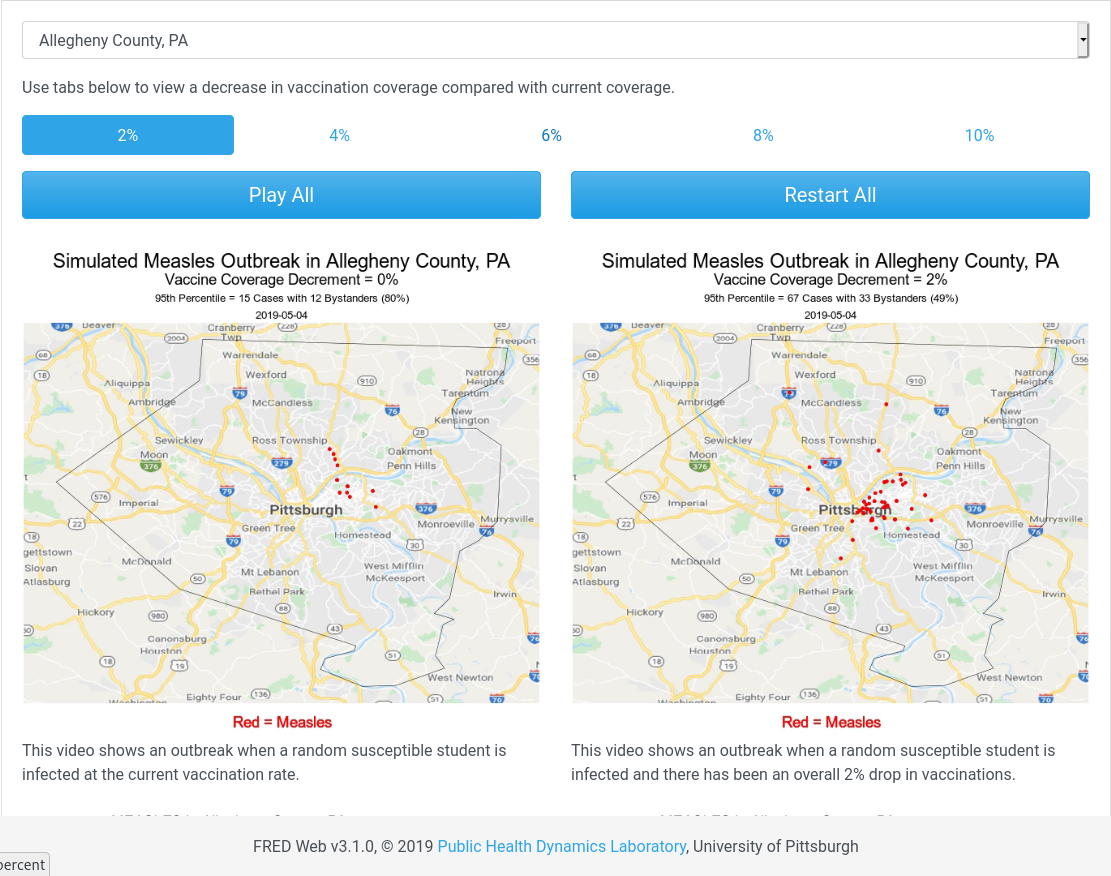
\includegraphics[width=0.5\textwidth]{./images/FRED_website.png}
  \end{figure}
  \begin{itemize}
  \item Developed at the University of Pittsburgh \citep{grefenstette2013}. 
  \item FRED is an agent-based model framework highly flexible and adaptable.
  \item We modified FRED to simulate COVID-19, some of the modifications include
    \begin{itemize}
      \item natural history of disease parameters,
      \item implemented adaptive non-pharmaceutical interventions.
    \end{itemize}
  \end{itemize}
    
\end{frame}



% =============================================================================%
\begin{frame}
  \frametitle{Agents can transmit the virus in specific places}

  \begin{figure}
    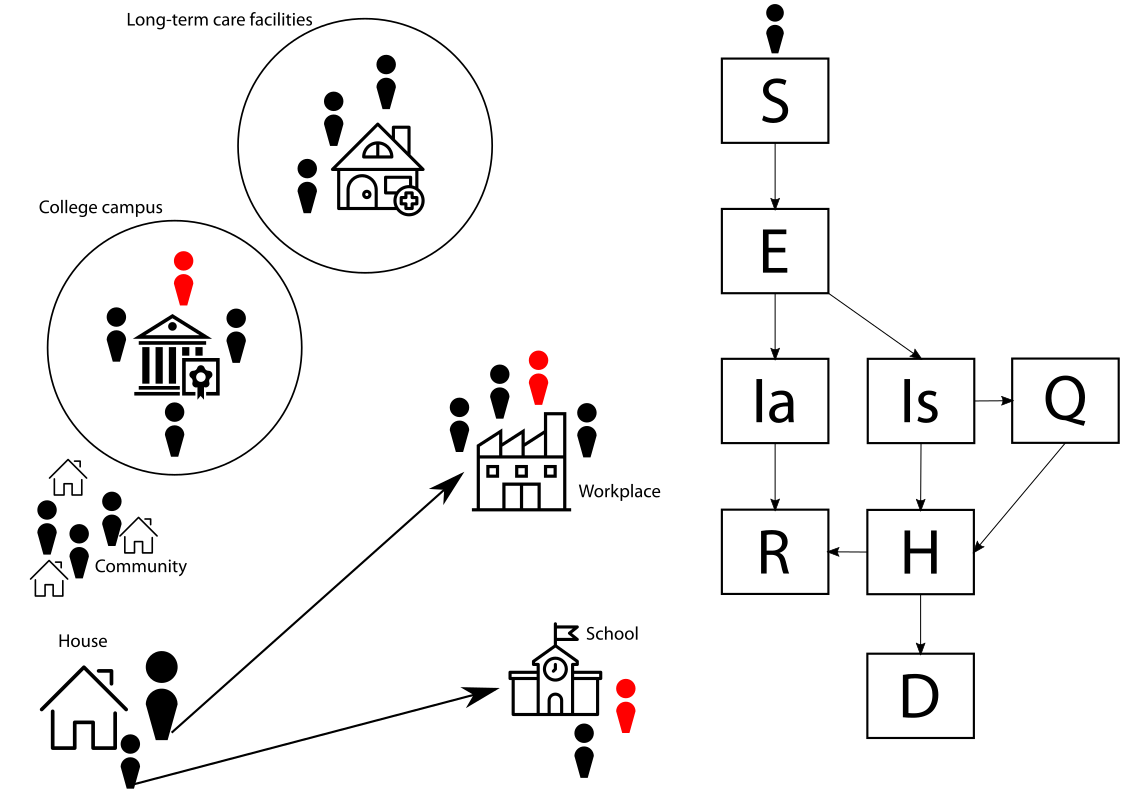
\includegraphics[width=0.95\textwidth]{./images/FRED_transmission.png}
  \end{figure}
  \begin{itemize}
  \item Infectious individuals might spread the virus where susceptible individuals visit the same places the same day.
  \end{itemize}    
\end{frame}



% =============================================================================%
\begin{frame}
  \frametitle{Probability of symptoms and death}
  \begin{figure}
    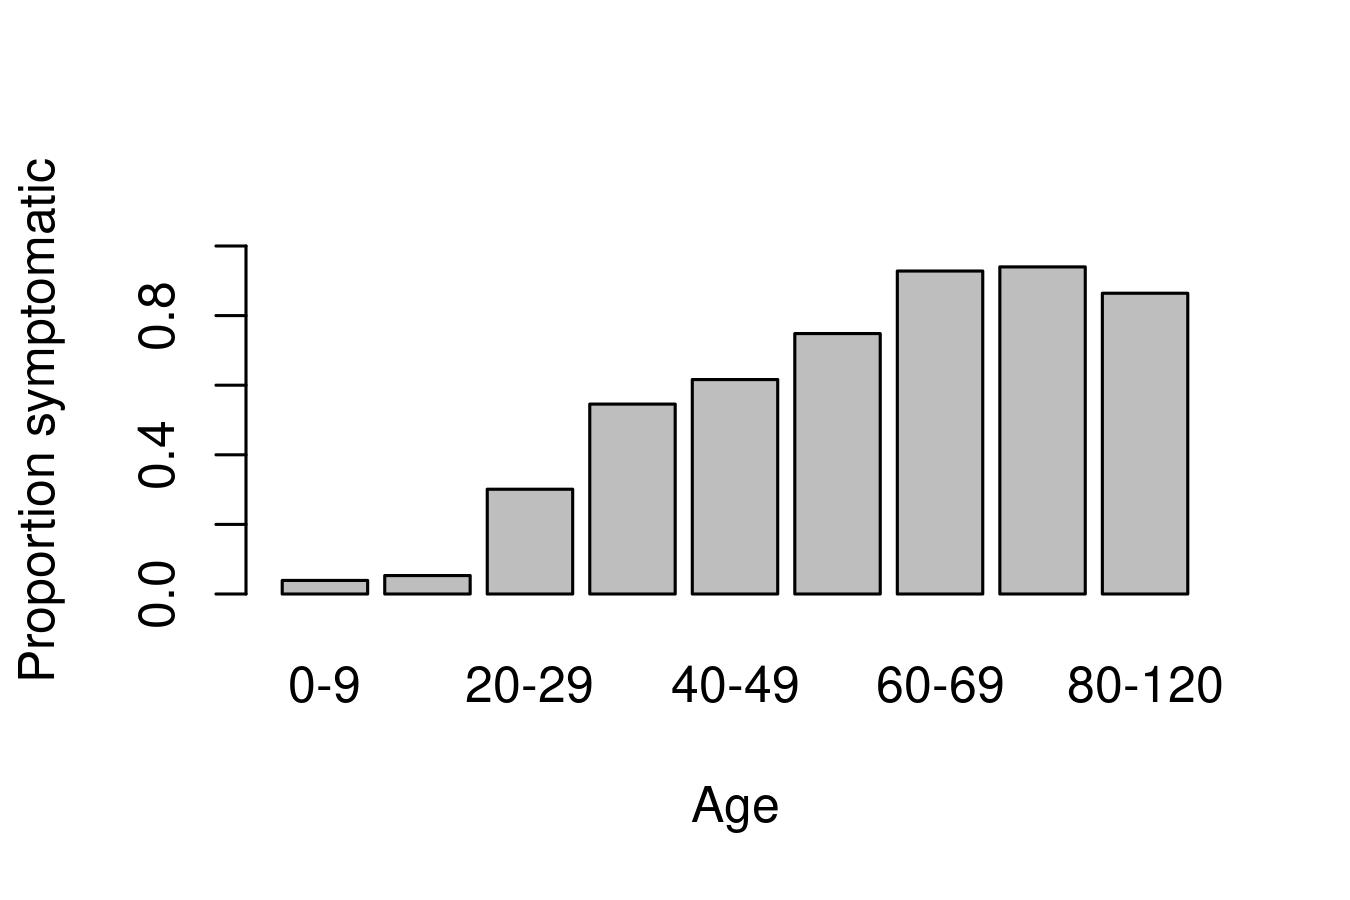
\includegraphics[width=0.5\textwidth]{./figures/manuscript_figure_age_symptoms.jpeg}
    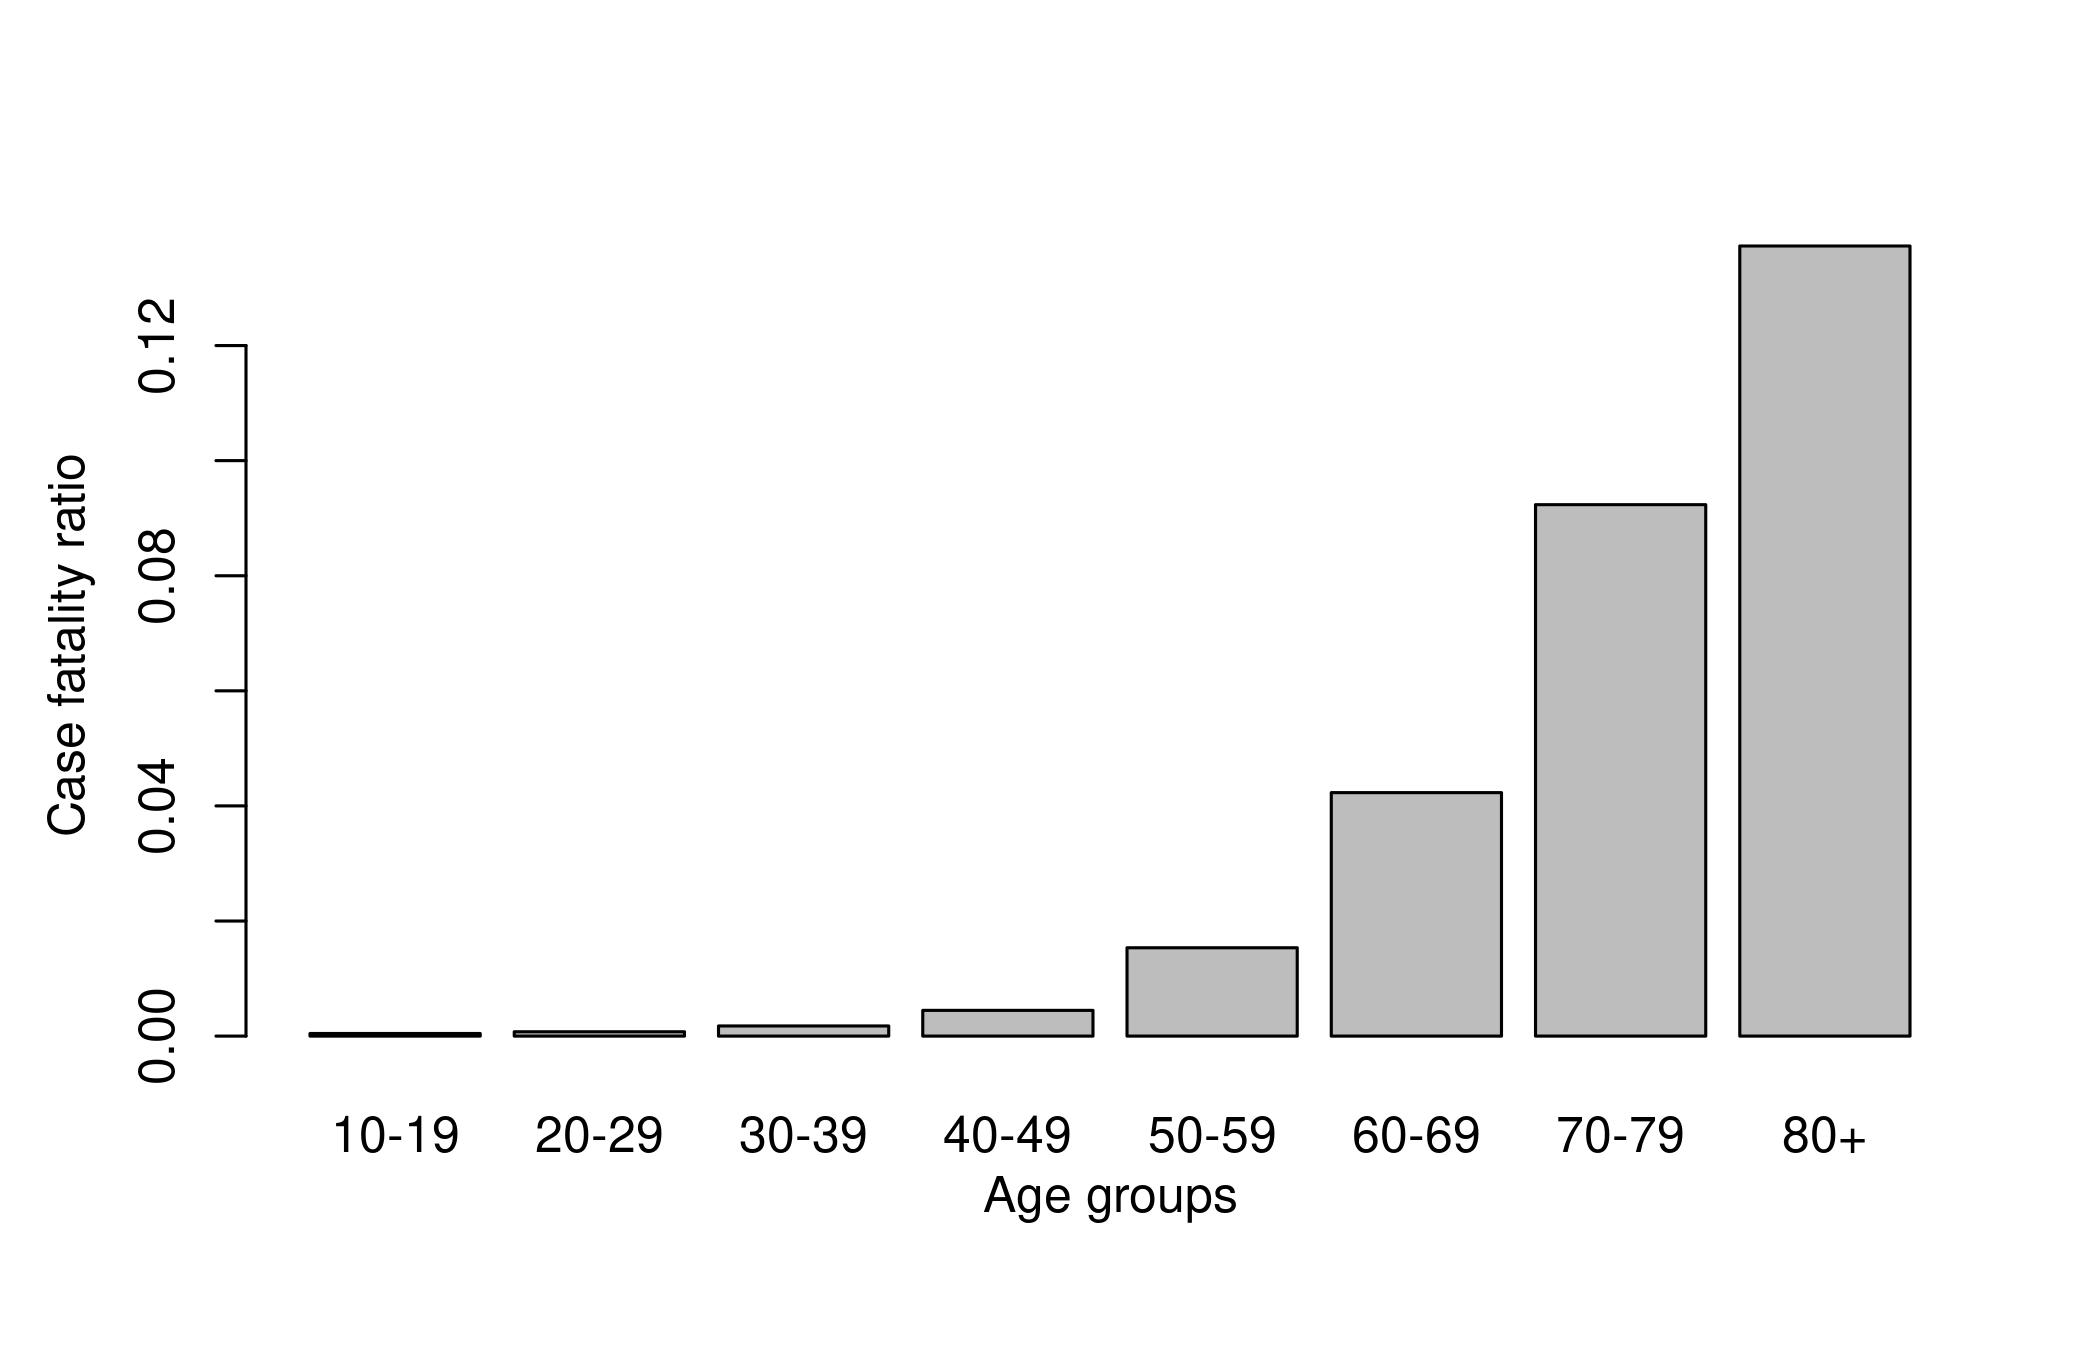
\includegraphics[width=0.5\textwidth]{./figures/manuscript_figure_age_CFR.jpeg}
    \caption{ From \citep{Verity2020_LancetID, ChinaCDC2020_weekly}.}
  \end{figure}
\end{frame}



% =============================================================================%
\begin{frame}
  \frametitle{Infectious period and duration of symptoms}
  \begin{figure}
    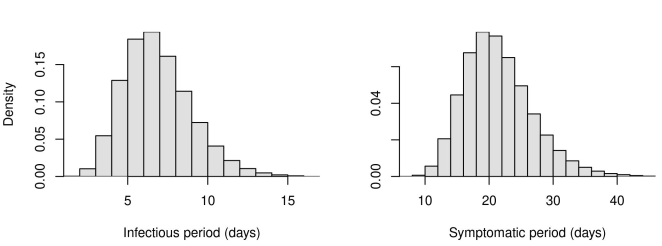
\includegraphics[width=0.8\textwidth]{./figures/manuscript_figure_parameter_periods.png}
    \caption{From \citep{He2020_Nature, Lauer2020_Annals,Bi2020_LancetID}}
  \end{figure}

\end{frame}

% =============================================================================%
\begin{frame}
  \frametitle{We focused on seven Midwest States}
   \begin{figure}
    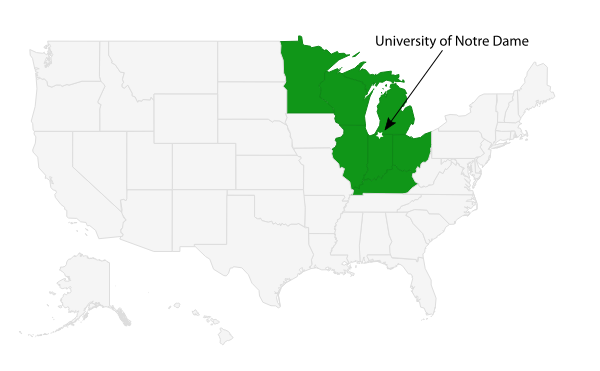
\includegraphics[width=0.8\textwidth]{./images/FRED_midwest_states_sim.png}
  \end{figure}

  \begin{itemize}
  \item We used deaths to calibrate the model parameters: shelter-in-place compliance, transmission efficiency, importation scaling, and asymptomatic relative infectivity.
  \item We simulate 2,000 parameter sets for each state.
  \end{itemize}    
\end{frame}


% =============================================================================%
\begin{frame}
  \frametitle{We estimated the trend in people staying at home from the google mobility trends}
  \begin{figure}
    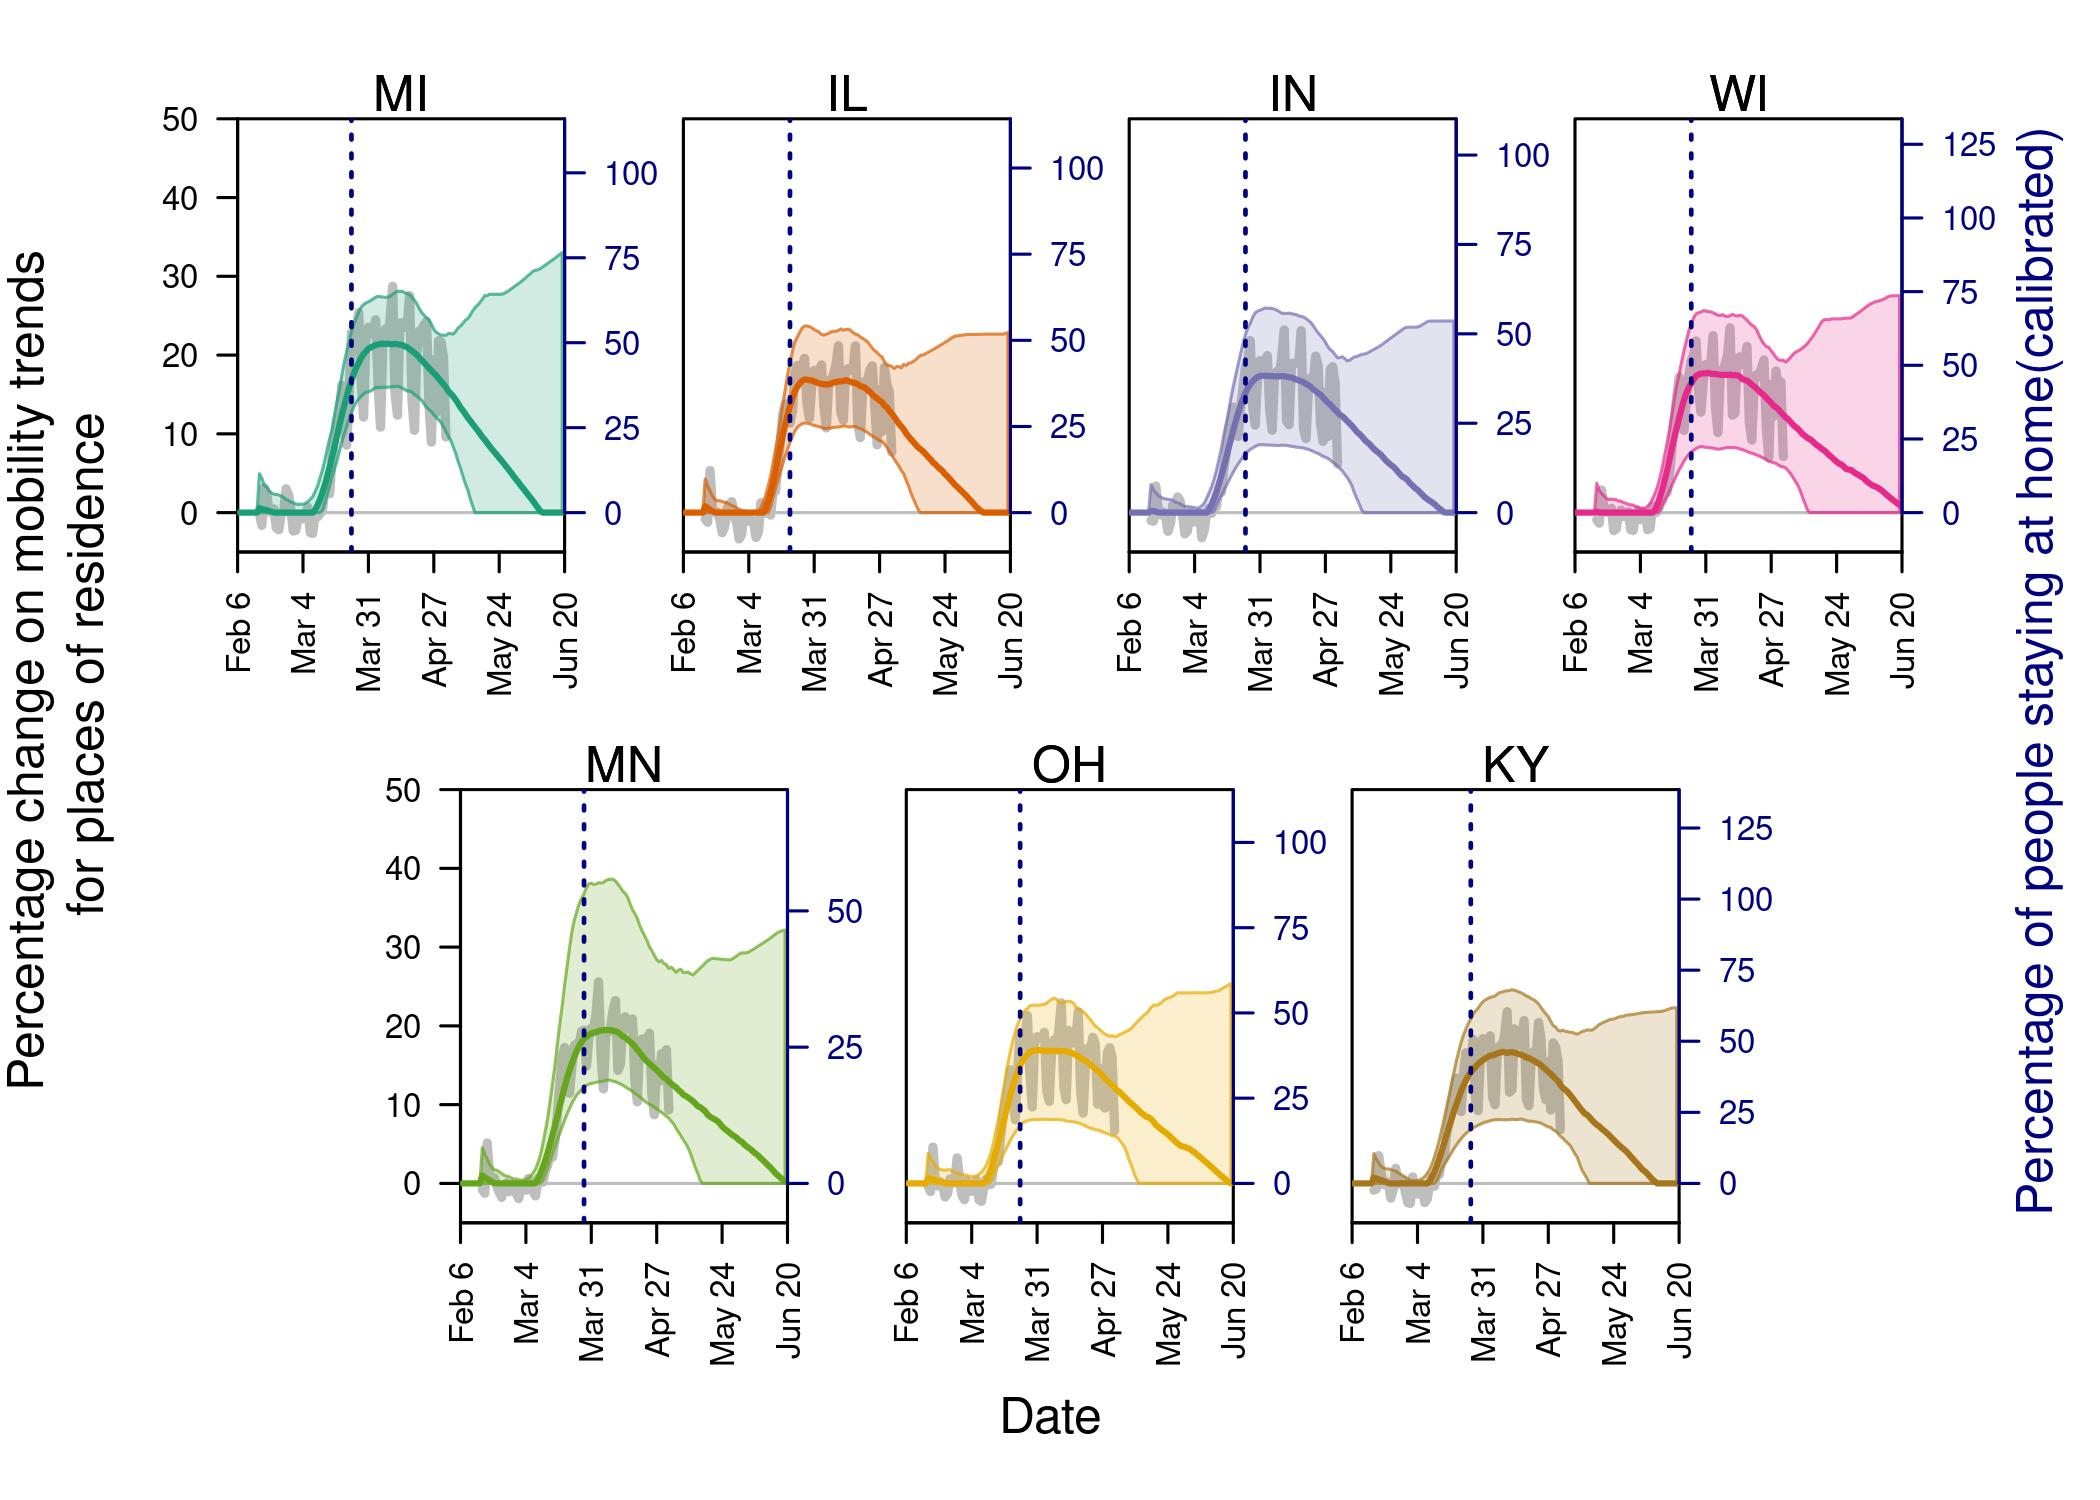
\includegraphics[width=0.89\textwidth]{../figures/report_figure_shelter_patterns.jpeg}
  \end{figure}
  \begin{itemize}
  \item After the data period, we assumed a linear trend for the forecasting horizon. 
  \end{itemize}    
\end{frame}


% =============================================================================%
\begin{frame}
  \frametitle{Calibrated parameters}
  \begin{figure}
    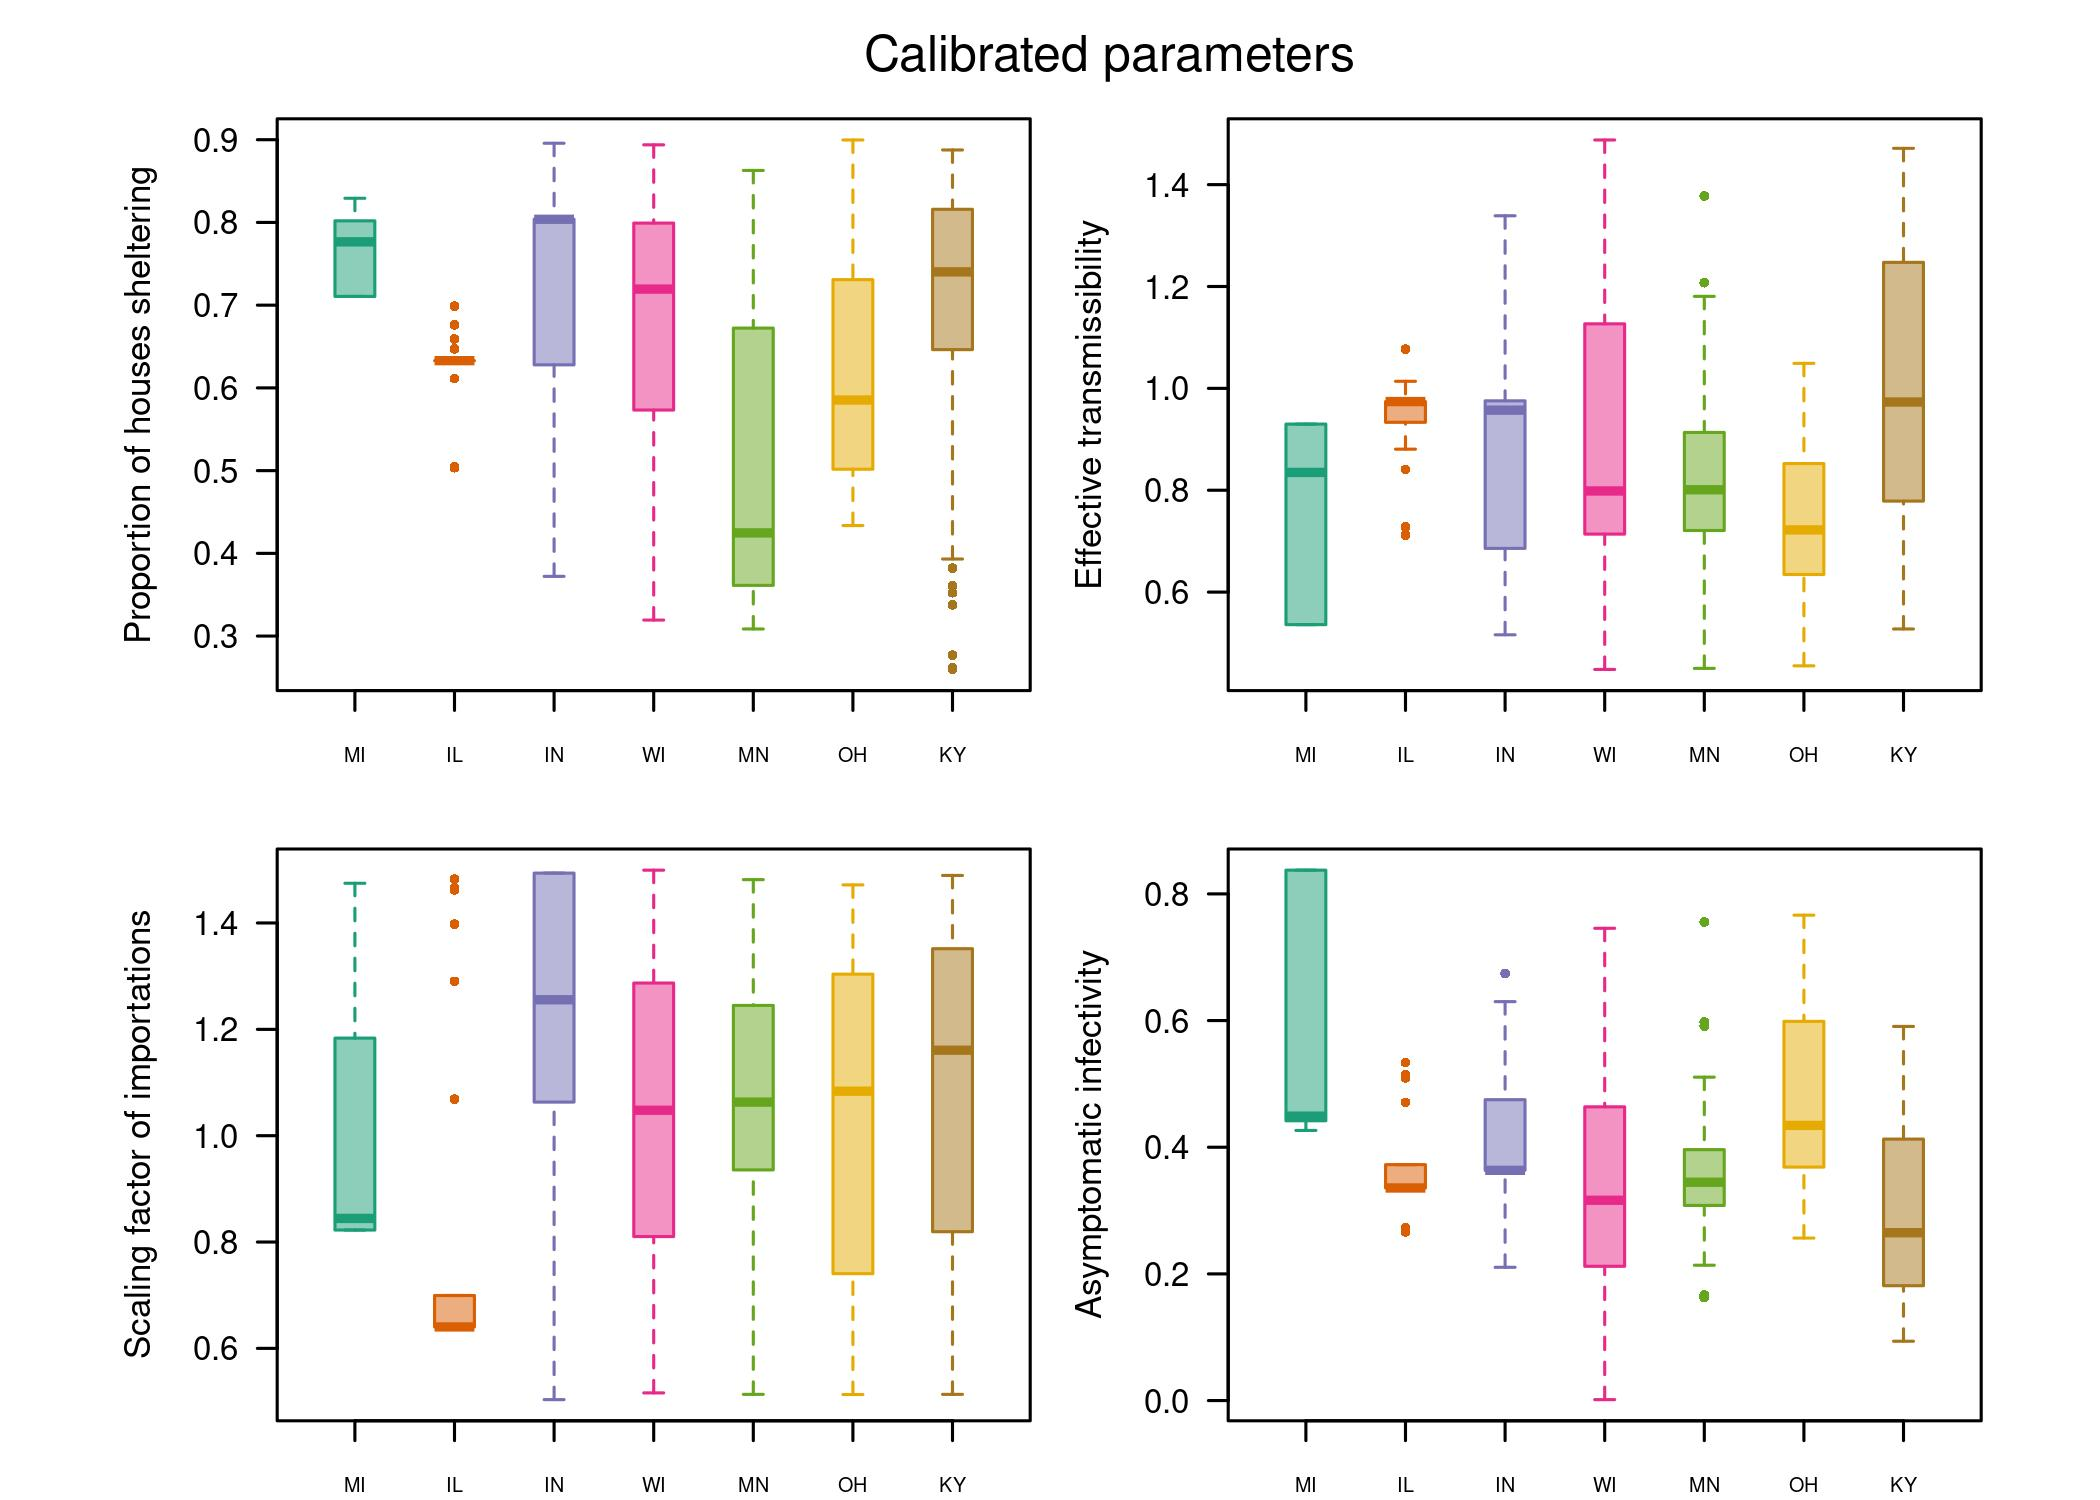
\includegraphics[width=0.89\textwidth]{../figures/report_figure_calibrated_parameters.jpeg}
  \end{figure}
  \begin{itemize}
  \item Parameters were estimated for each state.
  \end{itemize}    
\end{frame}

% =============================================================================%
\begin{frame}
  \frametitle{Model calibration to deaths}
  \begin{figure}
    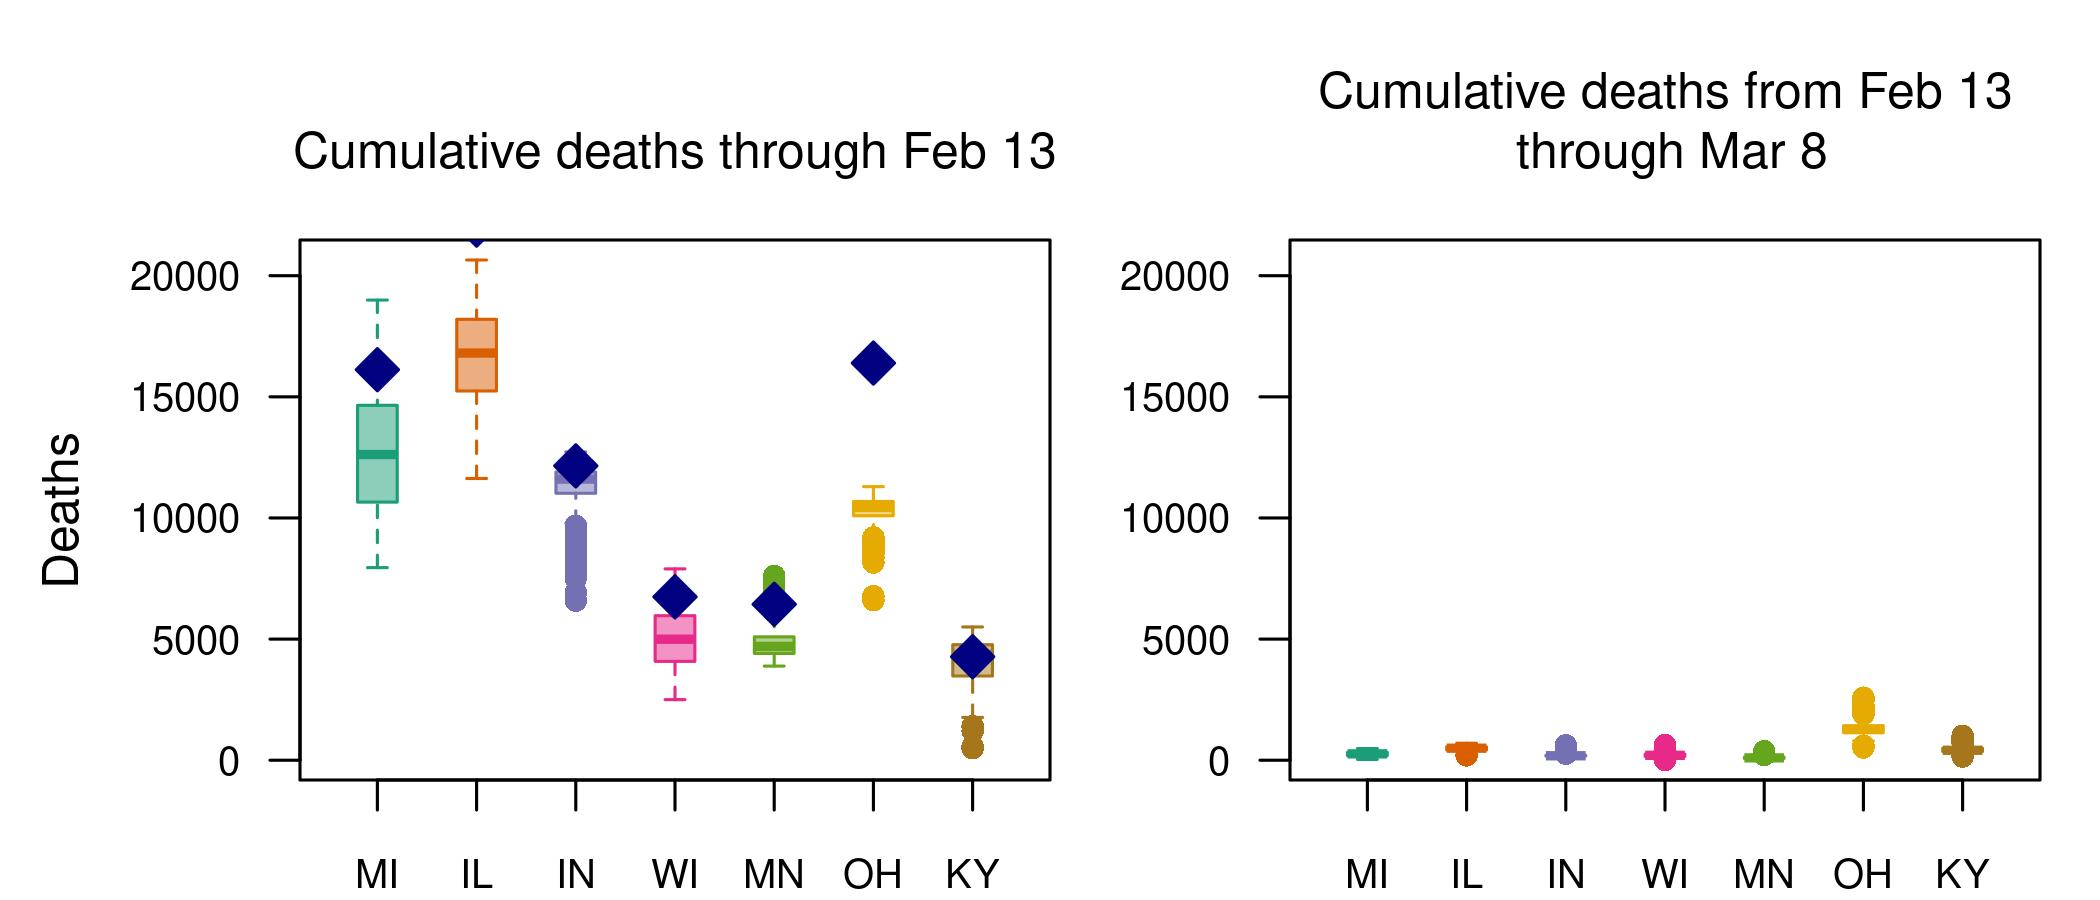
\includegraphics[width=0.89\textwidth]{../figures/report_figure_deaths_cumulative.jpeg}
  \end{figure}
  \begin{itemize}
  \item Cumulative deaths match the reported number of deaths in each state.
  \end{itemize}    
\end{frame}

% =============================================================================%
\begin{frame}
  \frametitle{Forecast: we assume shelter in place stays with the current trend, schools reopen.}
  \begin{figure}
    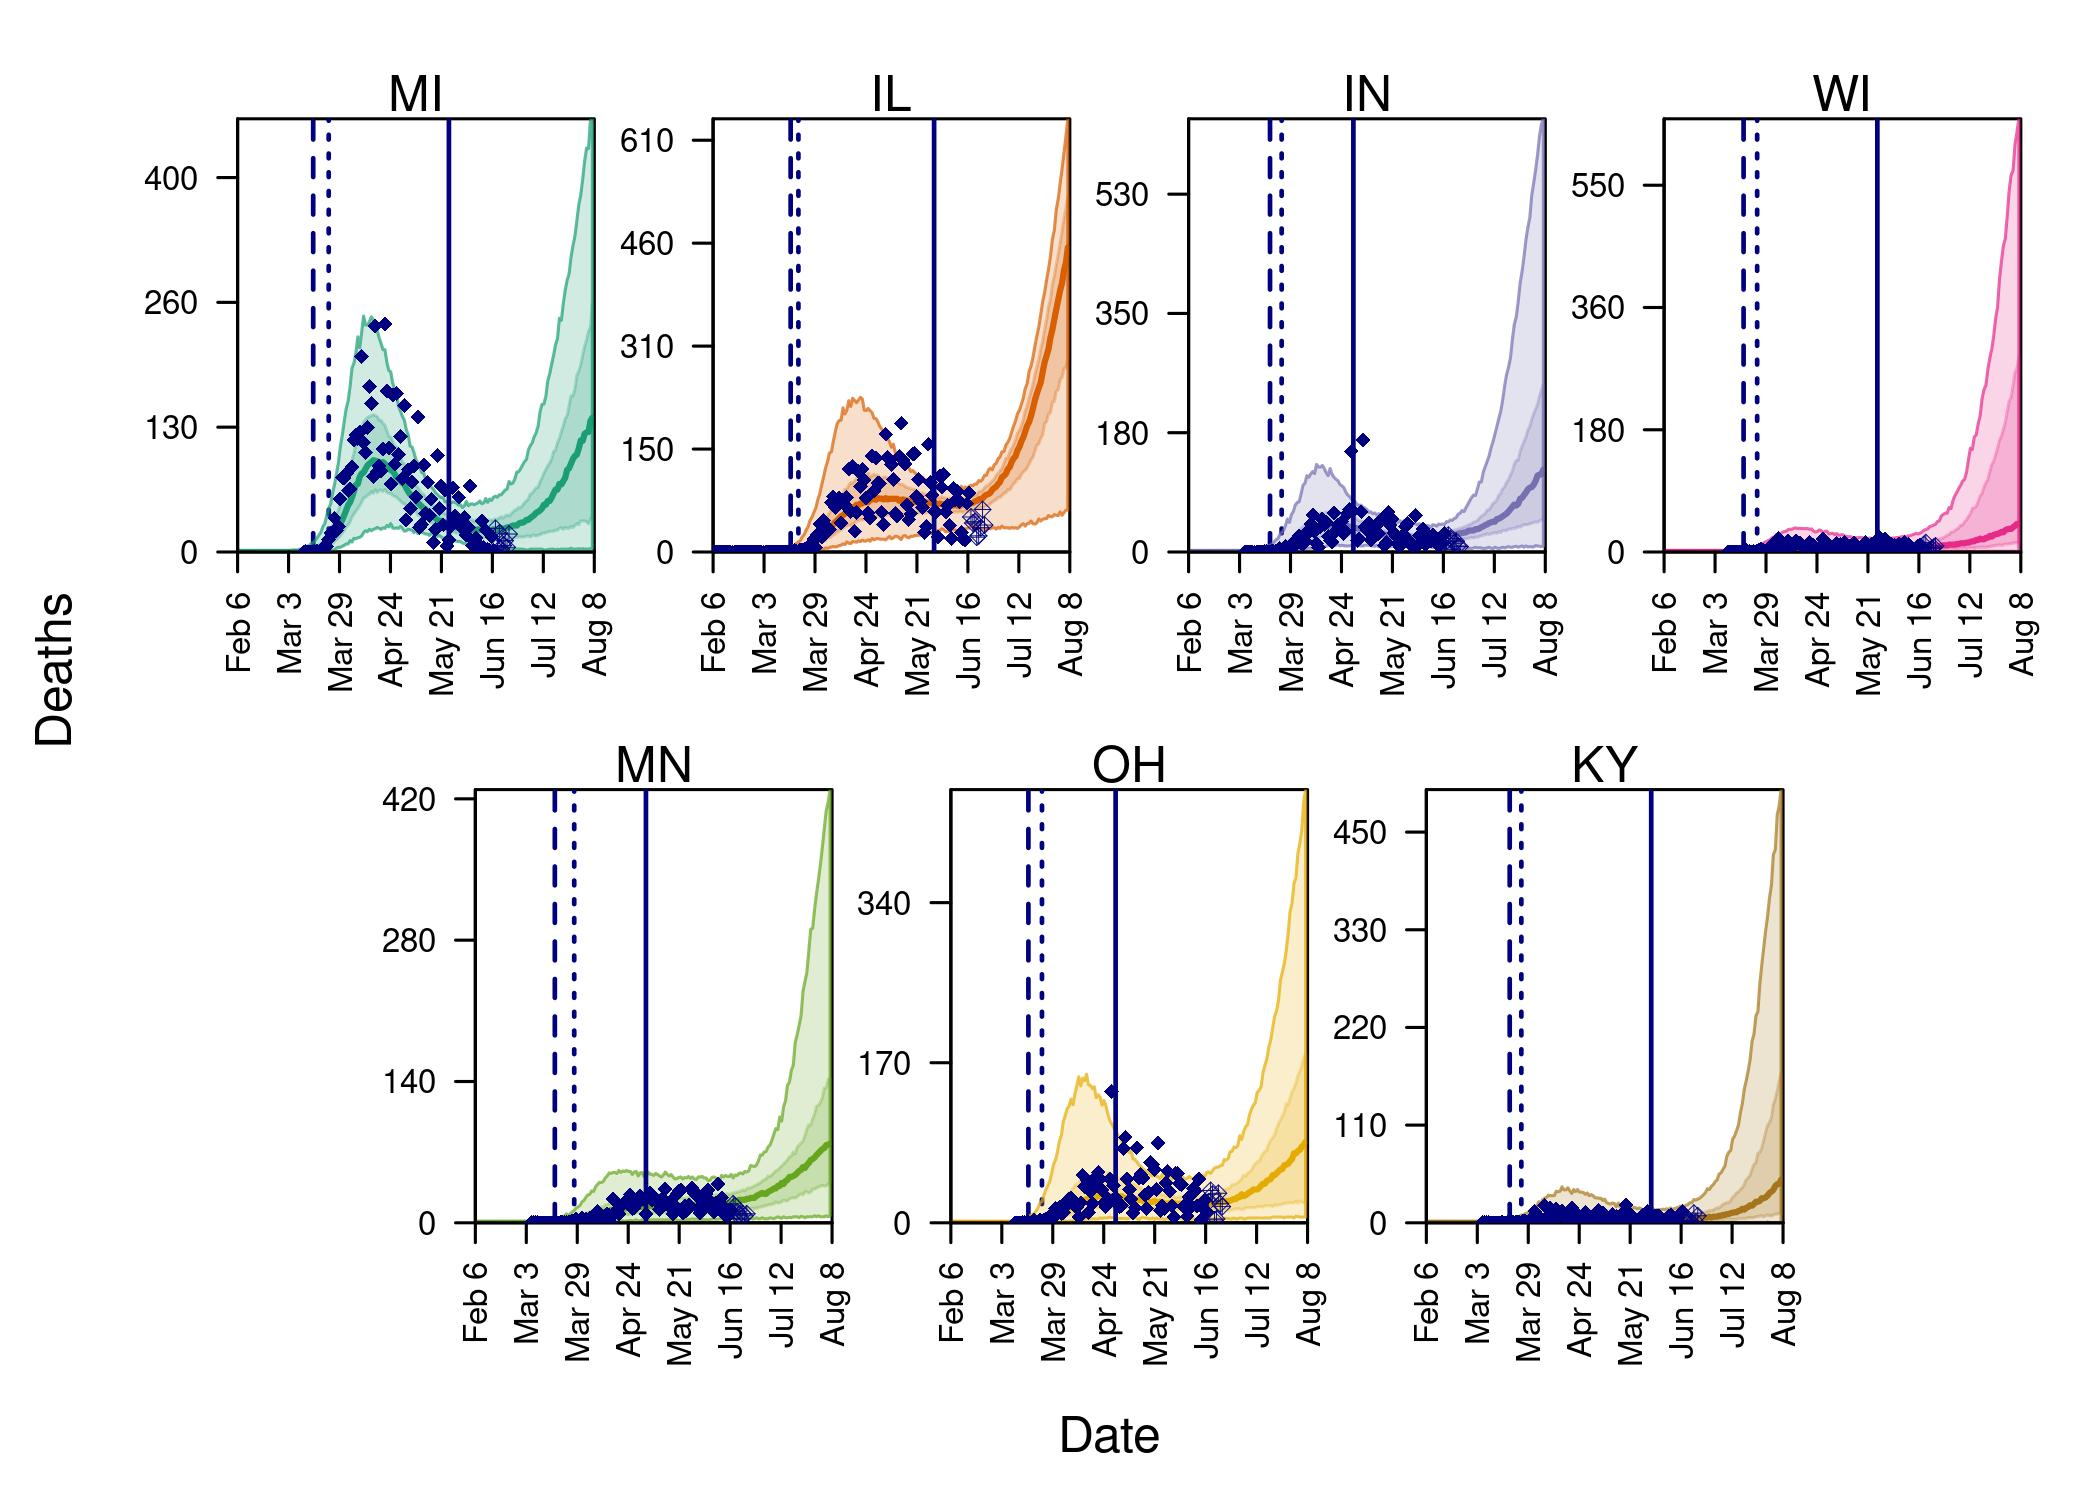
\includegraphics[width=0.85\textwidth]{../figures/report_figure_deaths_forecast.jpeg}
  \end{figure}
  \begin{itemize}
    \item Large impact of schools. Currently working on school reopen strategies. 
  \end{itemize}
\end{frame}



% =============================================================================%
\begin{frame}
  \frametitle{Reproduction number increases after interventions are relaxed and schools are open at full capacity}
    \begin{figure}
    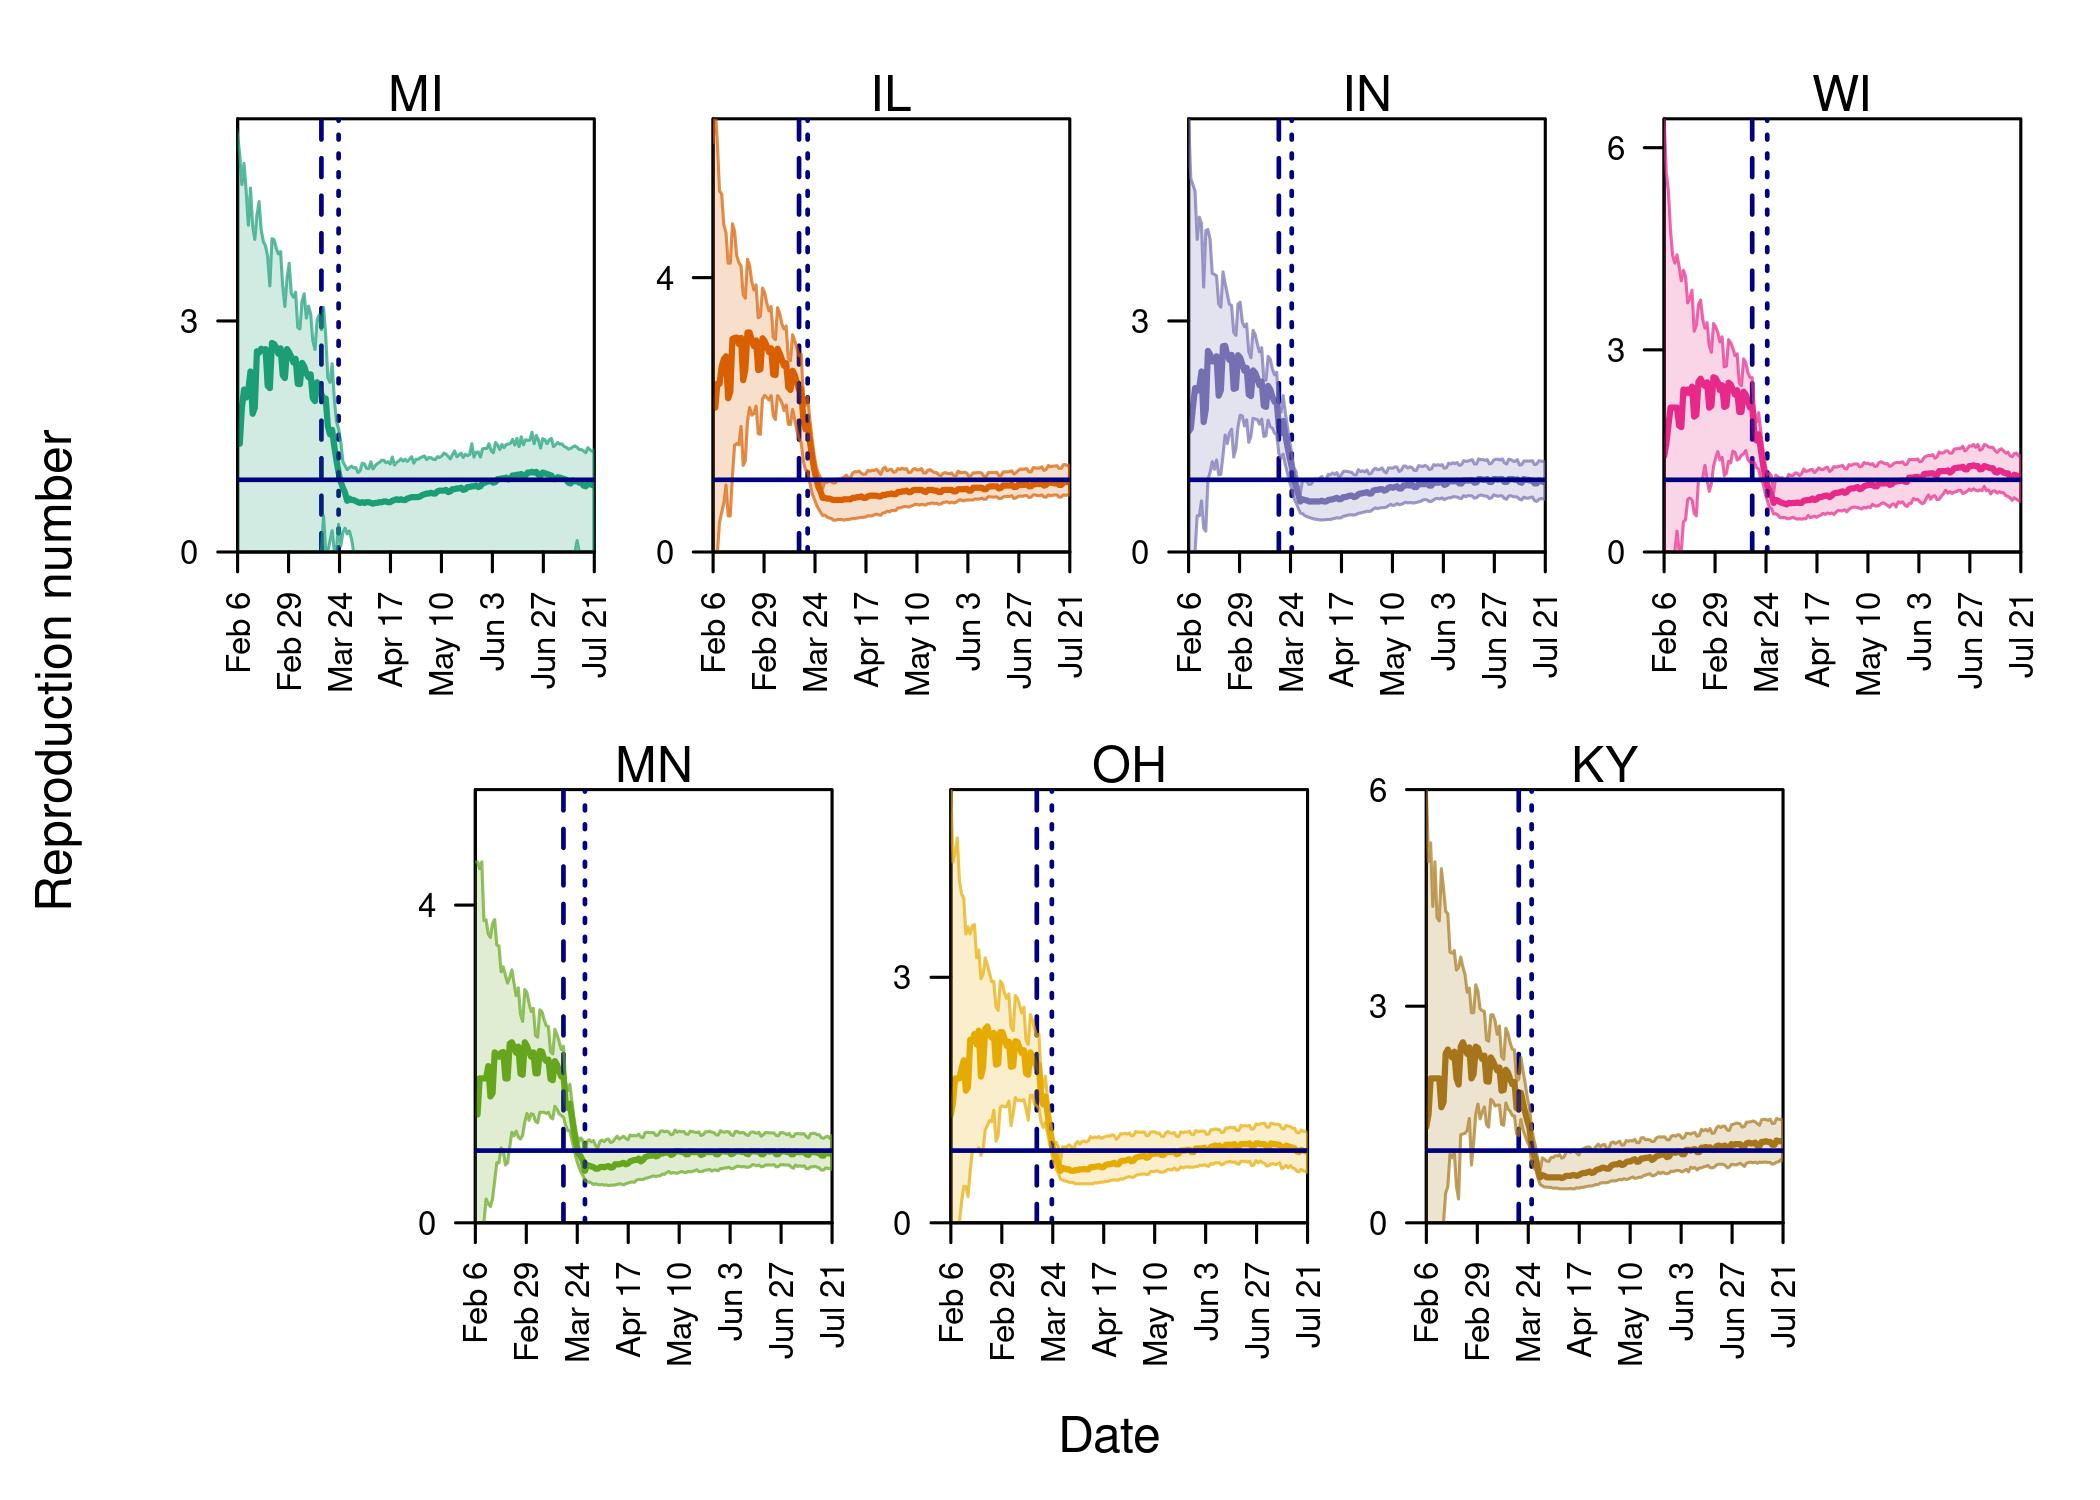
\includegraphics[width=0.95\textwidth]{../figures/report_figure_reproduction_number.jpeg}
  \end{figure}
\end{frame}

% =============================================================================%
\begin{frame}
  \frametitle{Evolution of forecast}
    \begin{figure}
    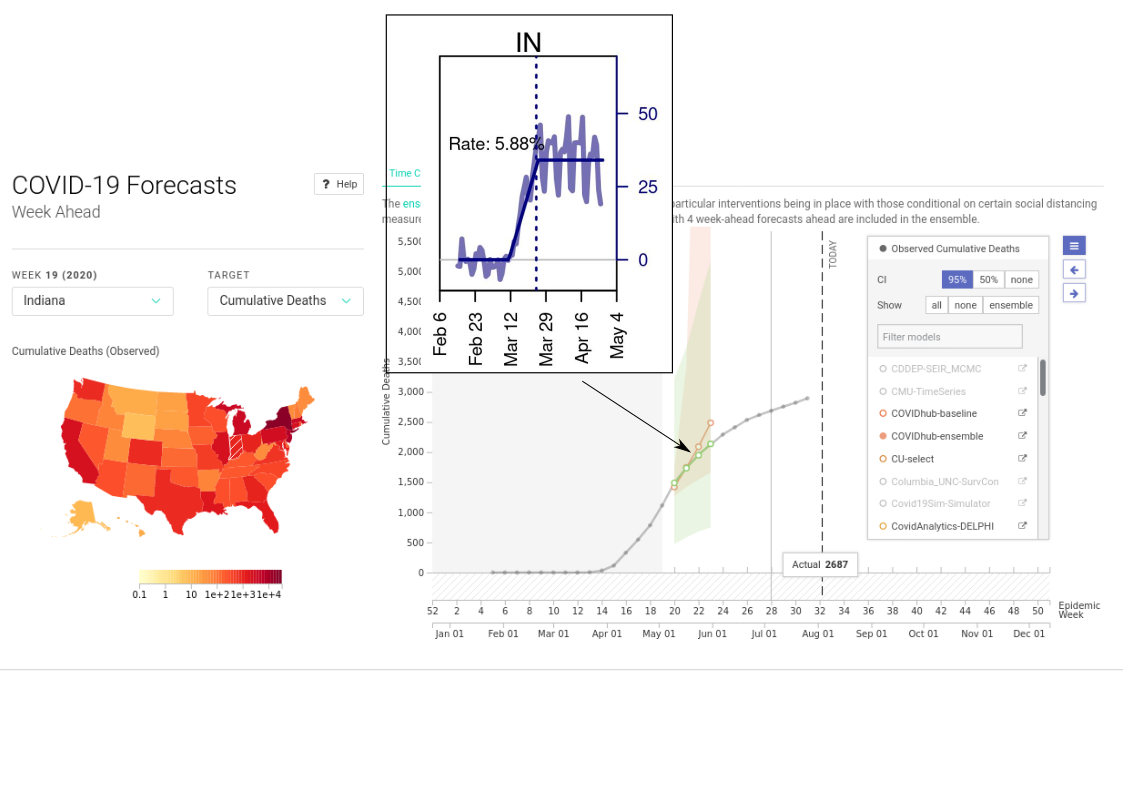
\includegraphics[width=0.95\textwidth]{./images/FRED_forecast_up_1.png}
  \end{figure}
\end{frame}

% =============================================================================%
\begin{frame}
  \frametitle{Evolution of forecast}
    \begin{figure}
    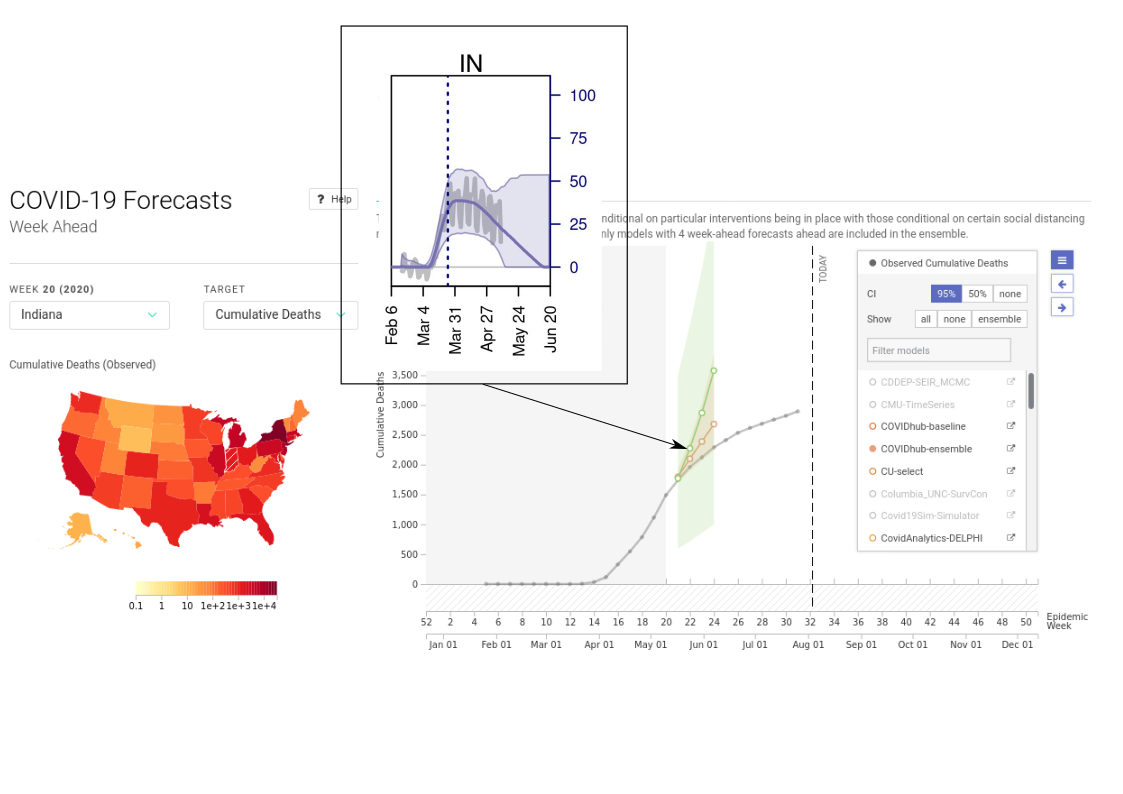
\includegraphics[width=0.95\textwidth]{./images/FRED_forecast_up_2.png}
  \end{figure}
\end{frame}

% =============================================================================%
\begin{frame}
  \frametitle{Evolution of forecast}
    \begin{figure}
    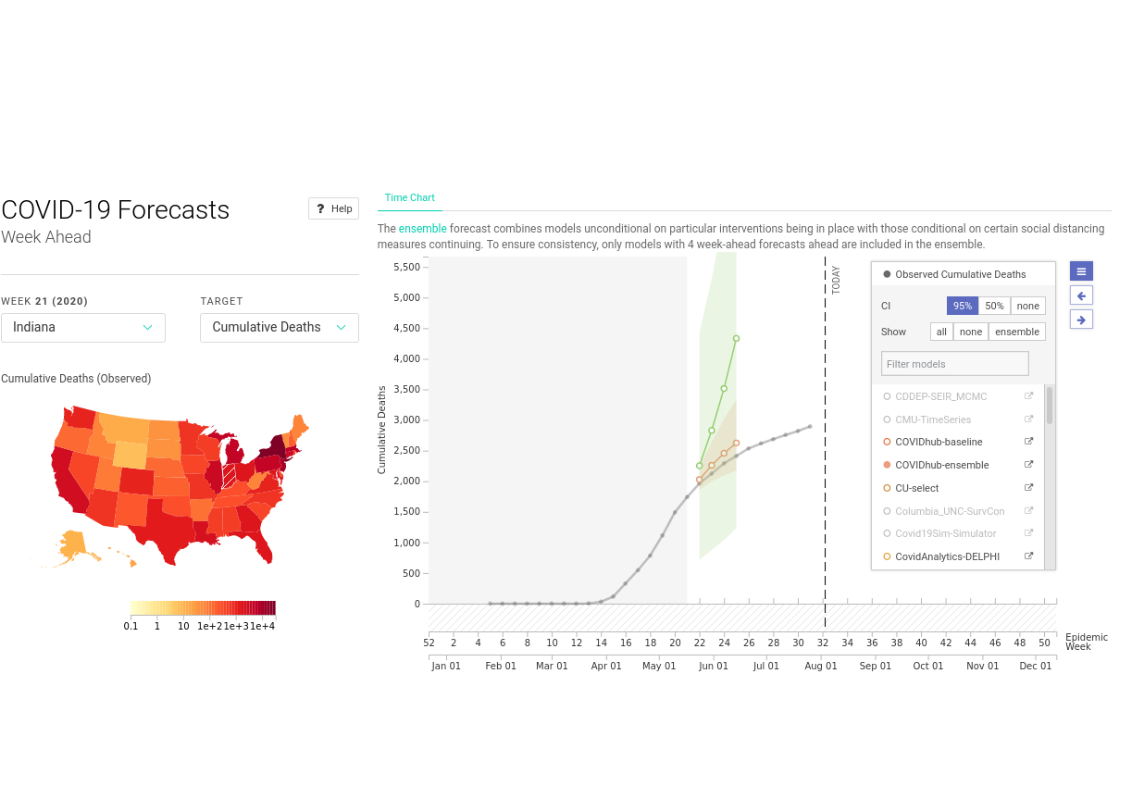
\includegraphics[width=0.95\textwidth]{./images/FRED_forecast_up_3.png}
  \end{figure}
\end{frame}

% =============================================================================%
\begin{frame}
  \frametitle{Evolution of forecast}
    \begin{figure}
    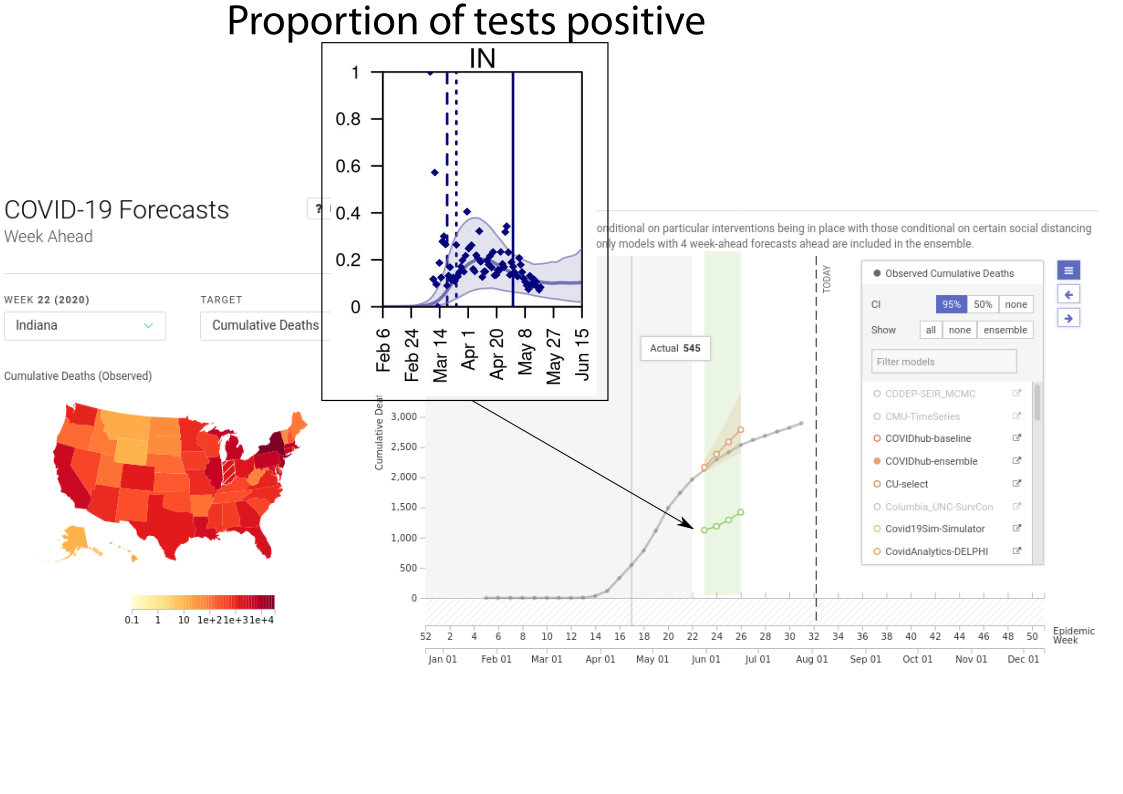
\includegraphics[width=0.95\textwidth]{./images/FRED_forecast_up_4.png}
  \end{figure}
\end{frame}

% =============================================================================%
\begin{frame}
  \frametitle{Evolution of forecast}
    \begin{figure}
    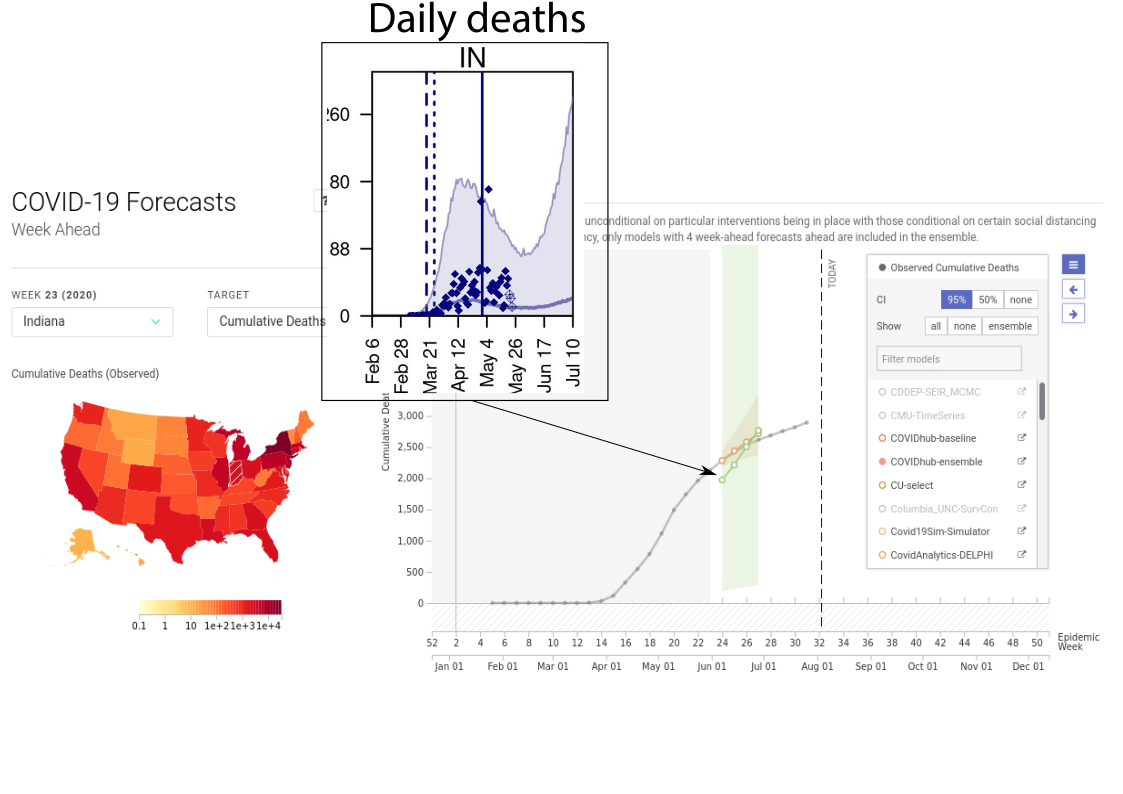
\includegraphics[width=0.95\textwidth]{./images/FRED_forecast_up_5.png}
  \end{figure}
\end{frame}

% =============================================================================%
\begin{frame}
  \frametitle{Evolution of forecast}
    \begin{figure}
    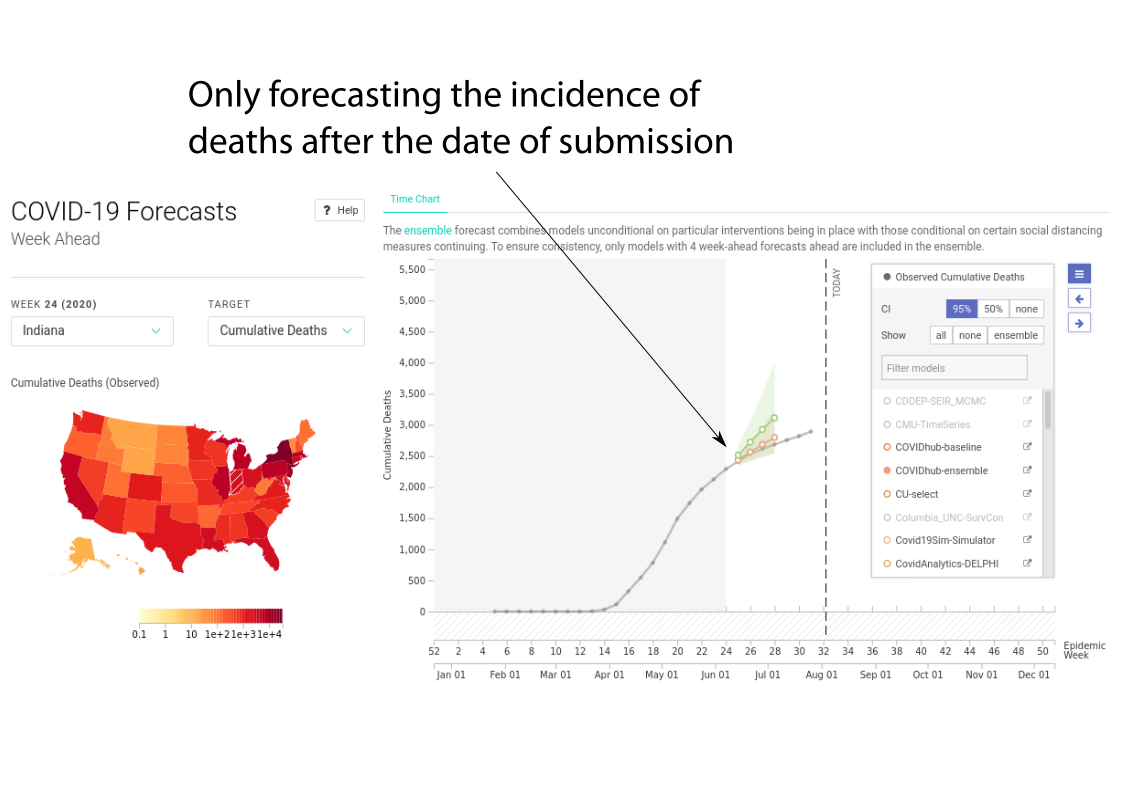
\includegraphics[width=0.95\textwidth]{./images/FRED_forecast_up_6.png}
  \end{figure}
\end{frame}

% =============================================================================%
\begin{frame}
  \frametitle{Evolution of forecast}
  \begin{figure}
    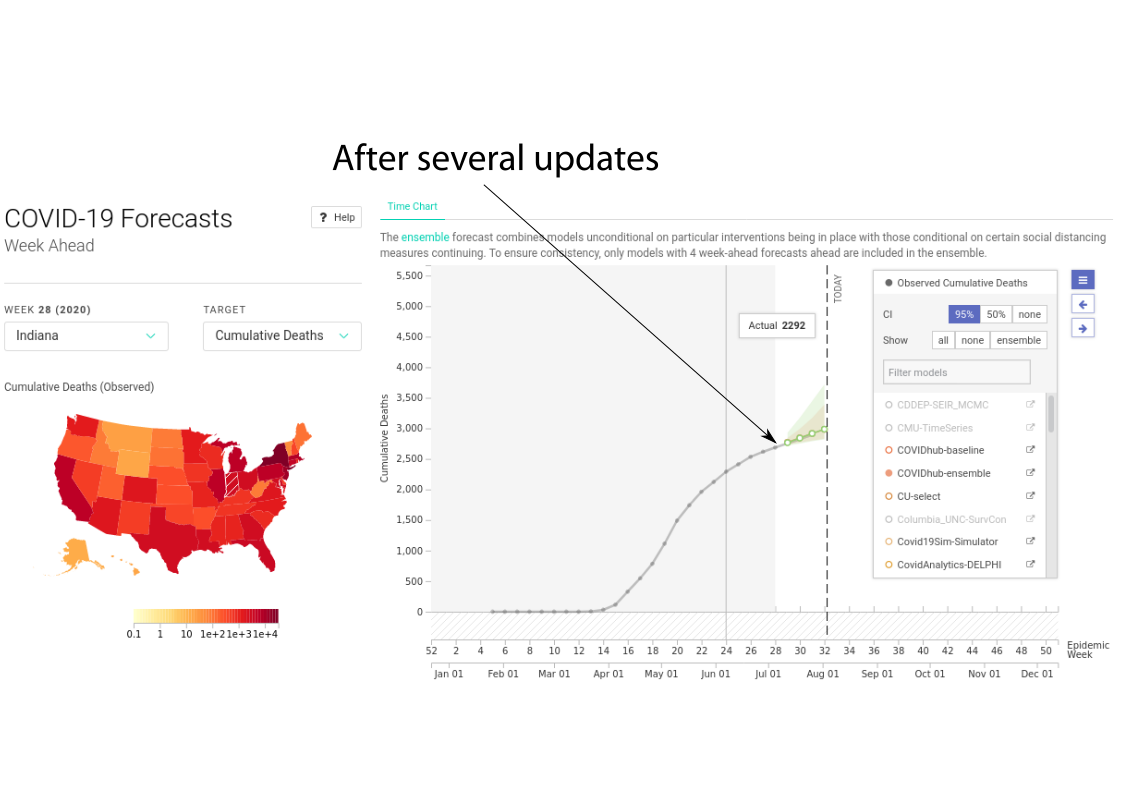
\includegraphics[width=0.95\textwidth]{./images/FRED_forecast_up_7.png}
  \end{figure}
\end{frame}

% % =============================================================================%
% \begin{frame}
%   \frametitle{To improve fit in Indiana, we are adding more data sources}
%   \begin{figure}
%     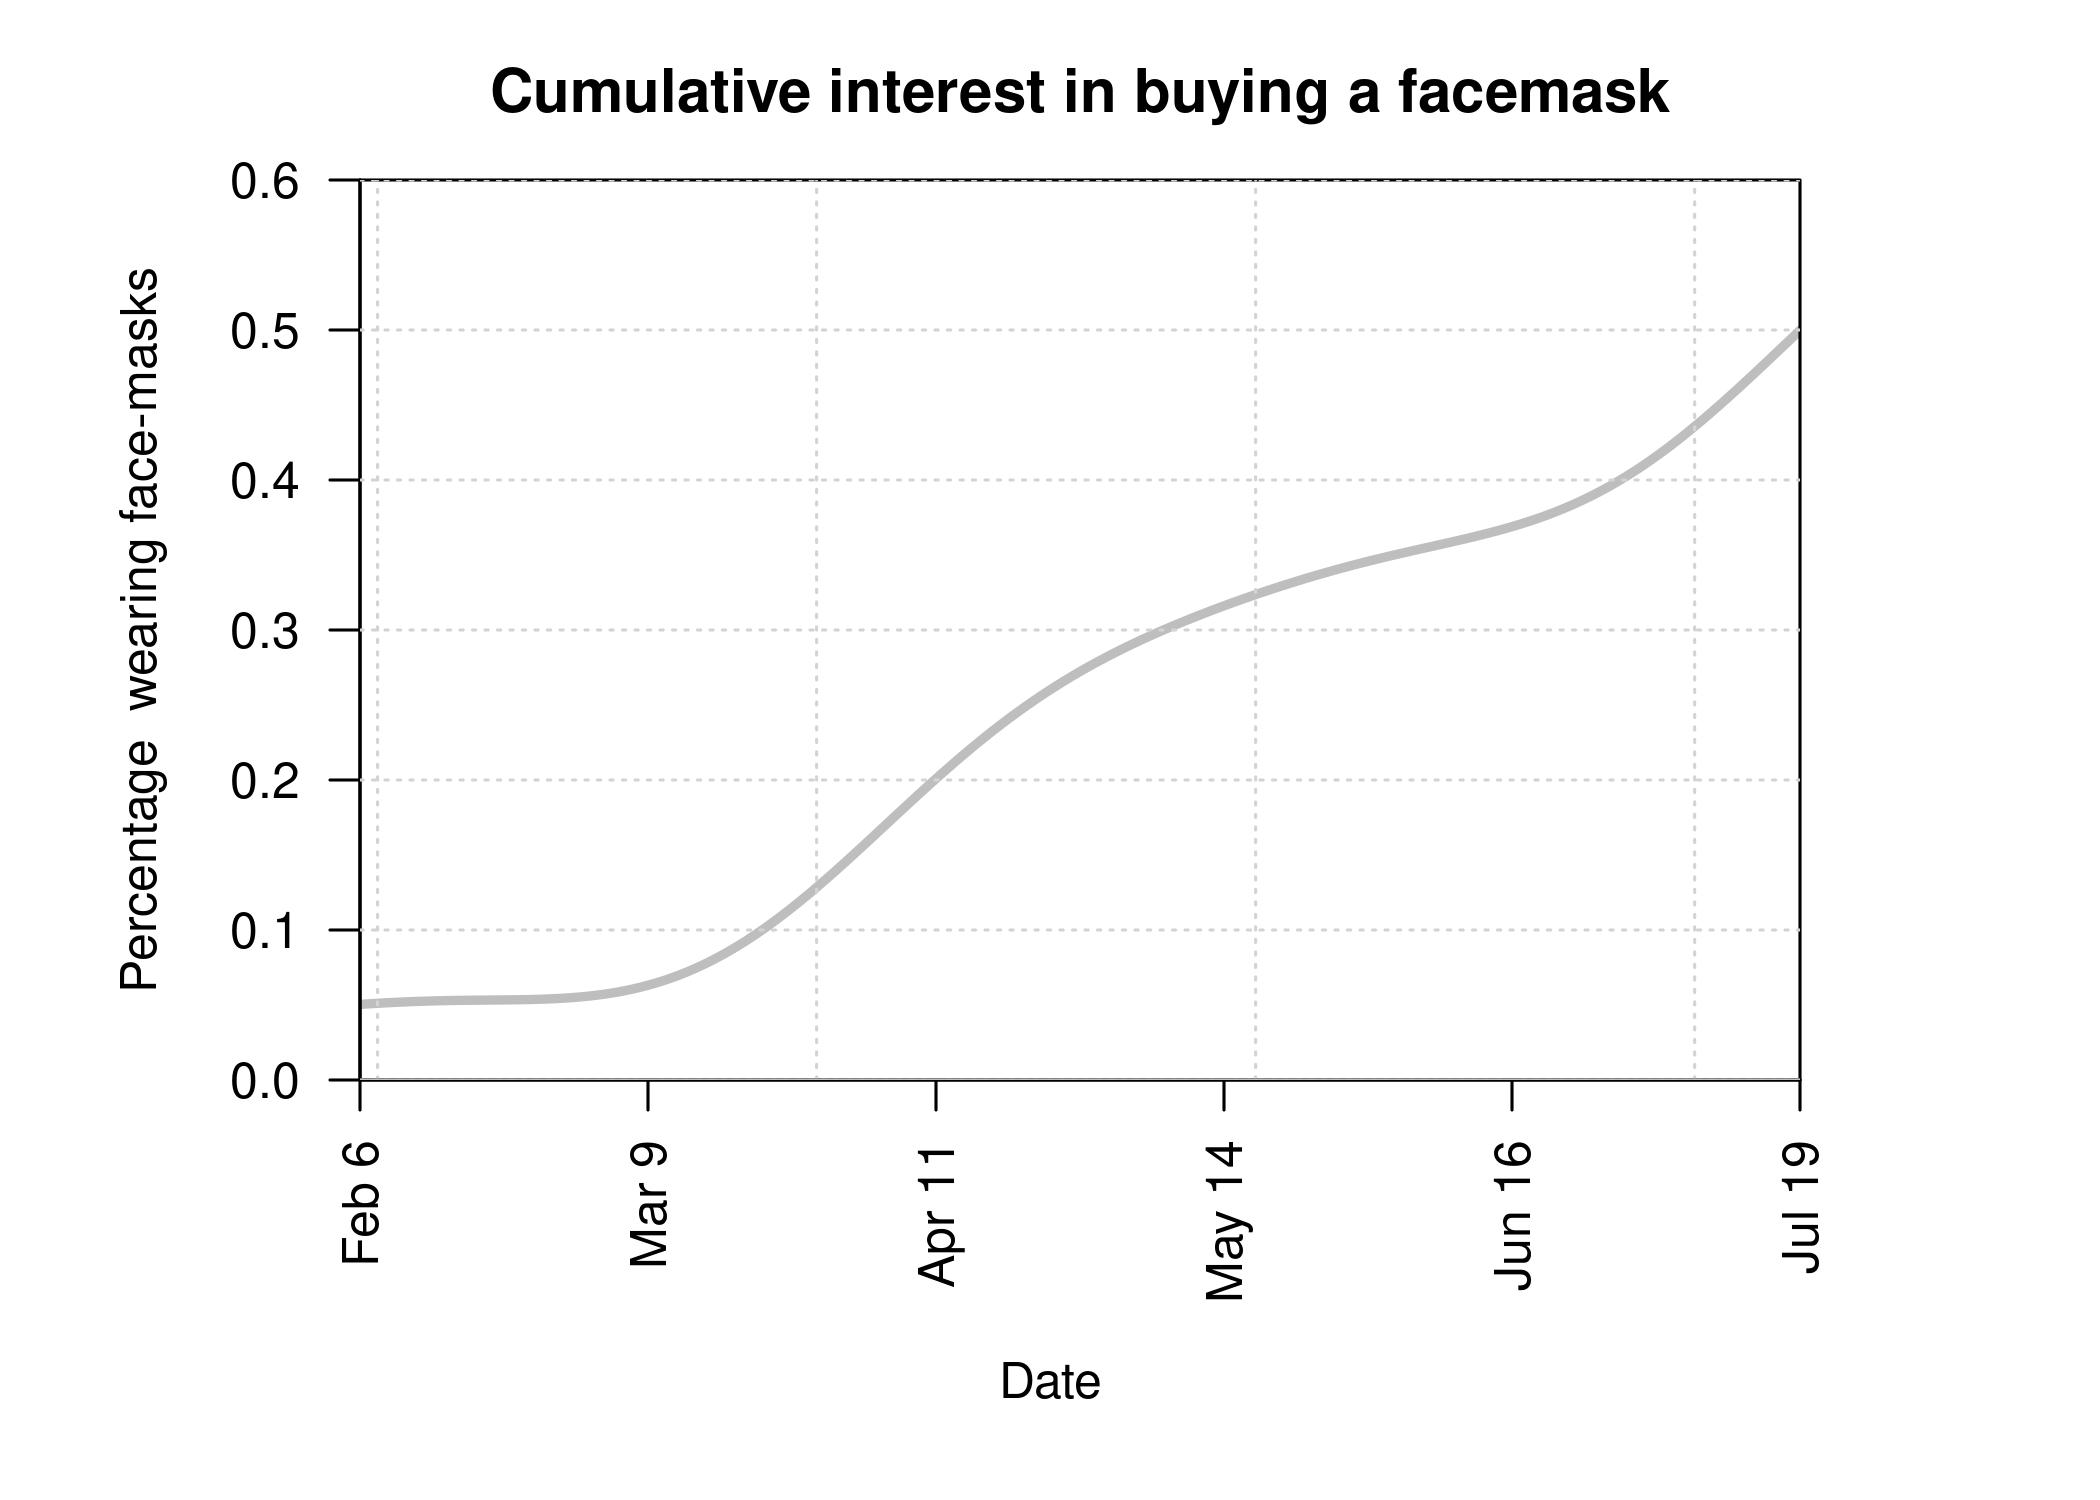
\includegraphics[width=0.95\textwidth]{./figures/figure_facemask_compliance.jpeg}
%   \end{figure}
% \end{frame}



% =============================================================================%
\begin{frame}
  \frametitle{To improve fit in Indiana, we included age-structure data}
    \begin{figure}
    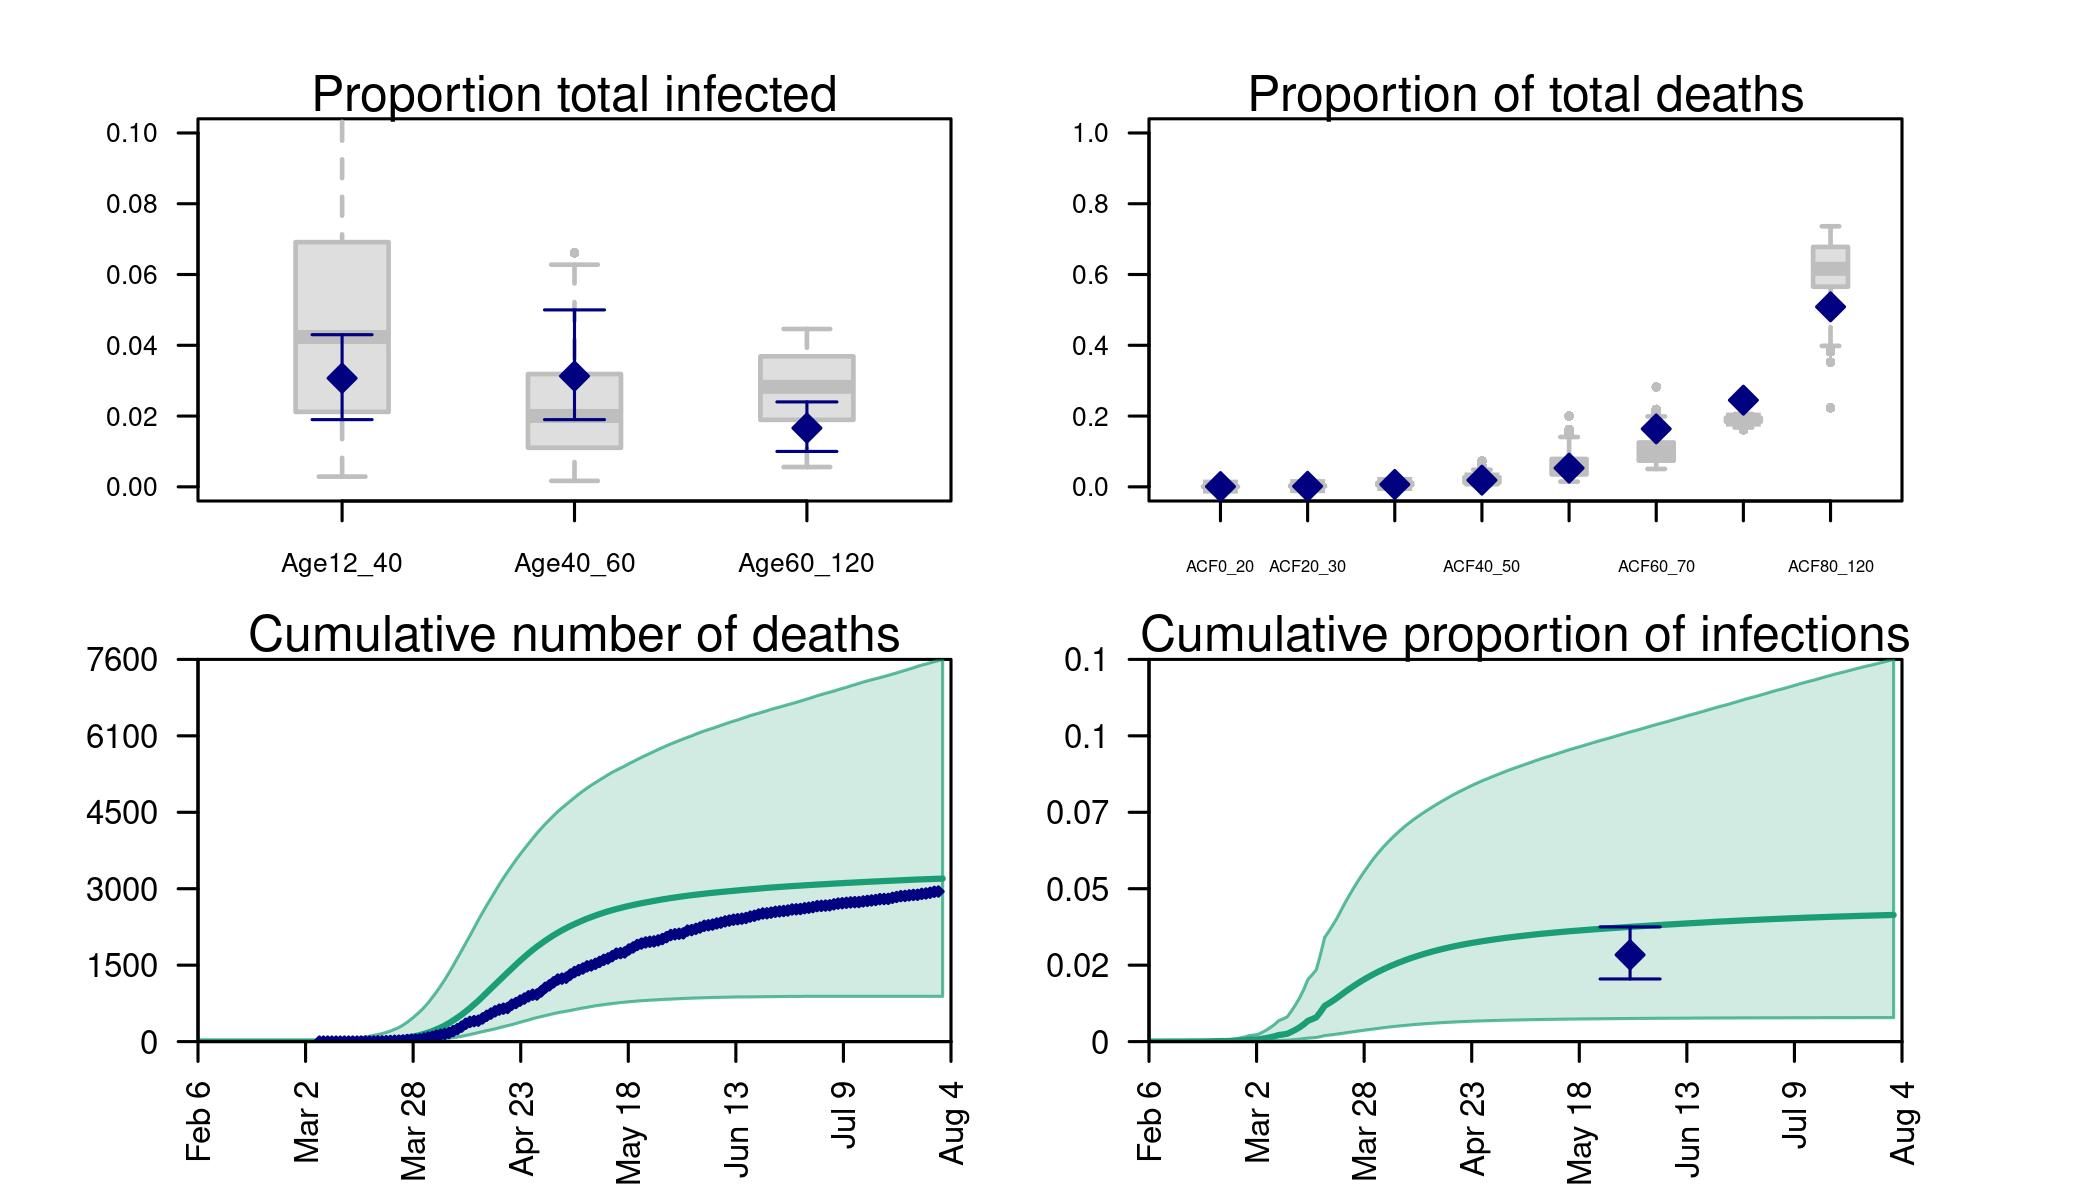
\includegraphics[width=0.95\textwidth]{./figures/manuscript_figure_age_deaths.jpeg}
  \end{figure}
  \begin{itemize}
  \item Lower susceptibility in <20 based on \citep{Davies2020_NatMed}. 
  \item We used the number of cases in long-term care facilities and estimated importations to these facilities.
  \item We calibrated the model to the age structure of deaths in Indiana and validated to serological studies.
  \end{itemize}
  
\end{frame}

% =============================================================================%
\begin{frame}
  \frametitle{To improve fit in Indiana, we included testing and hospitalizations}
  \begin{figure}
    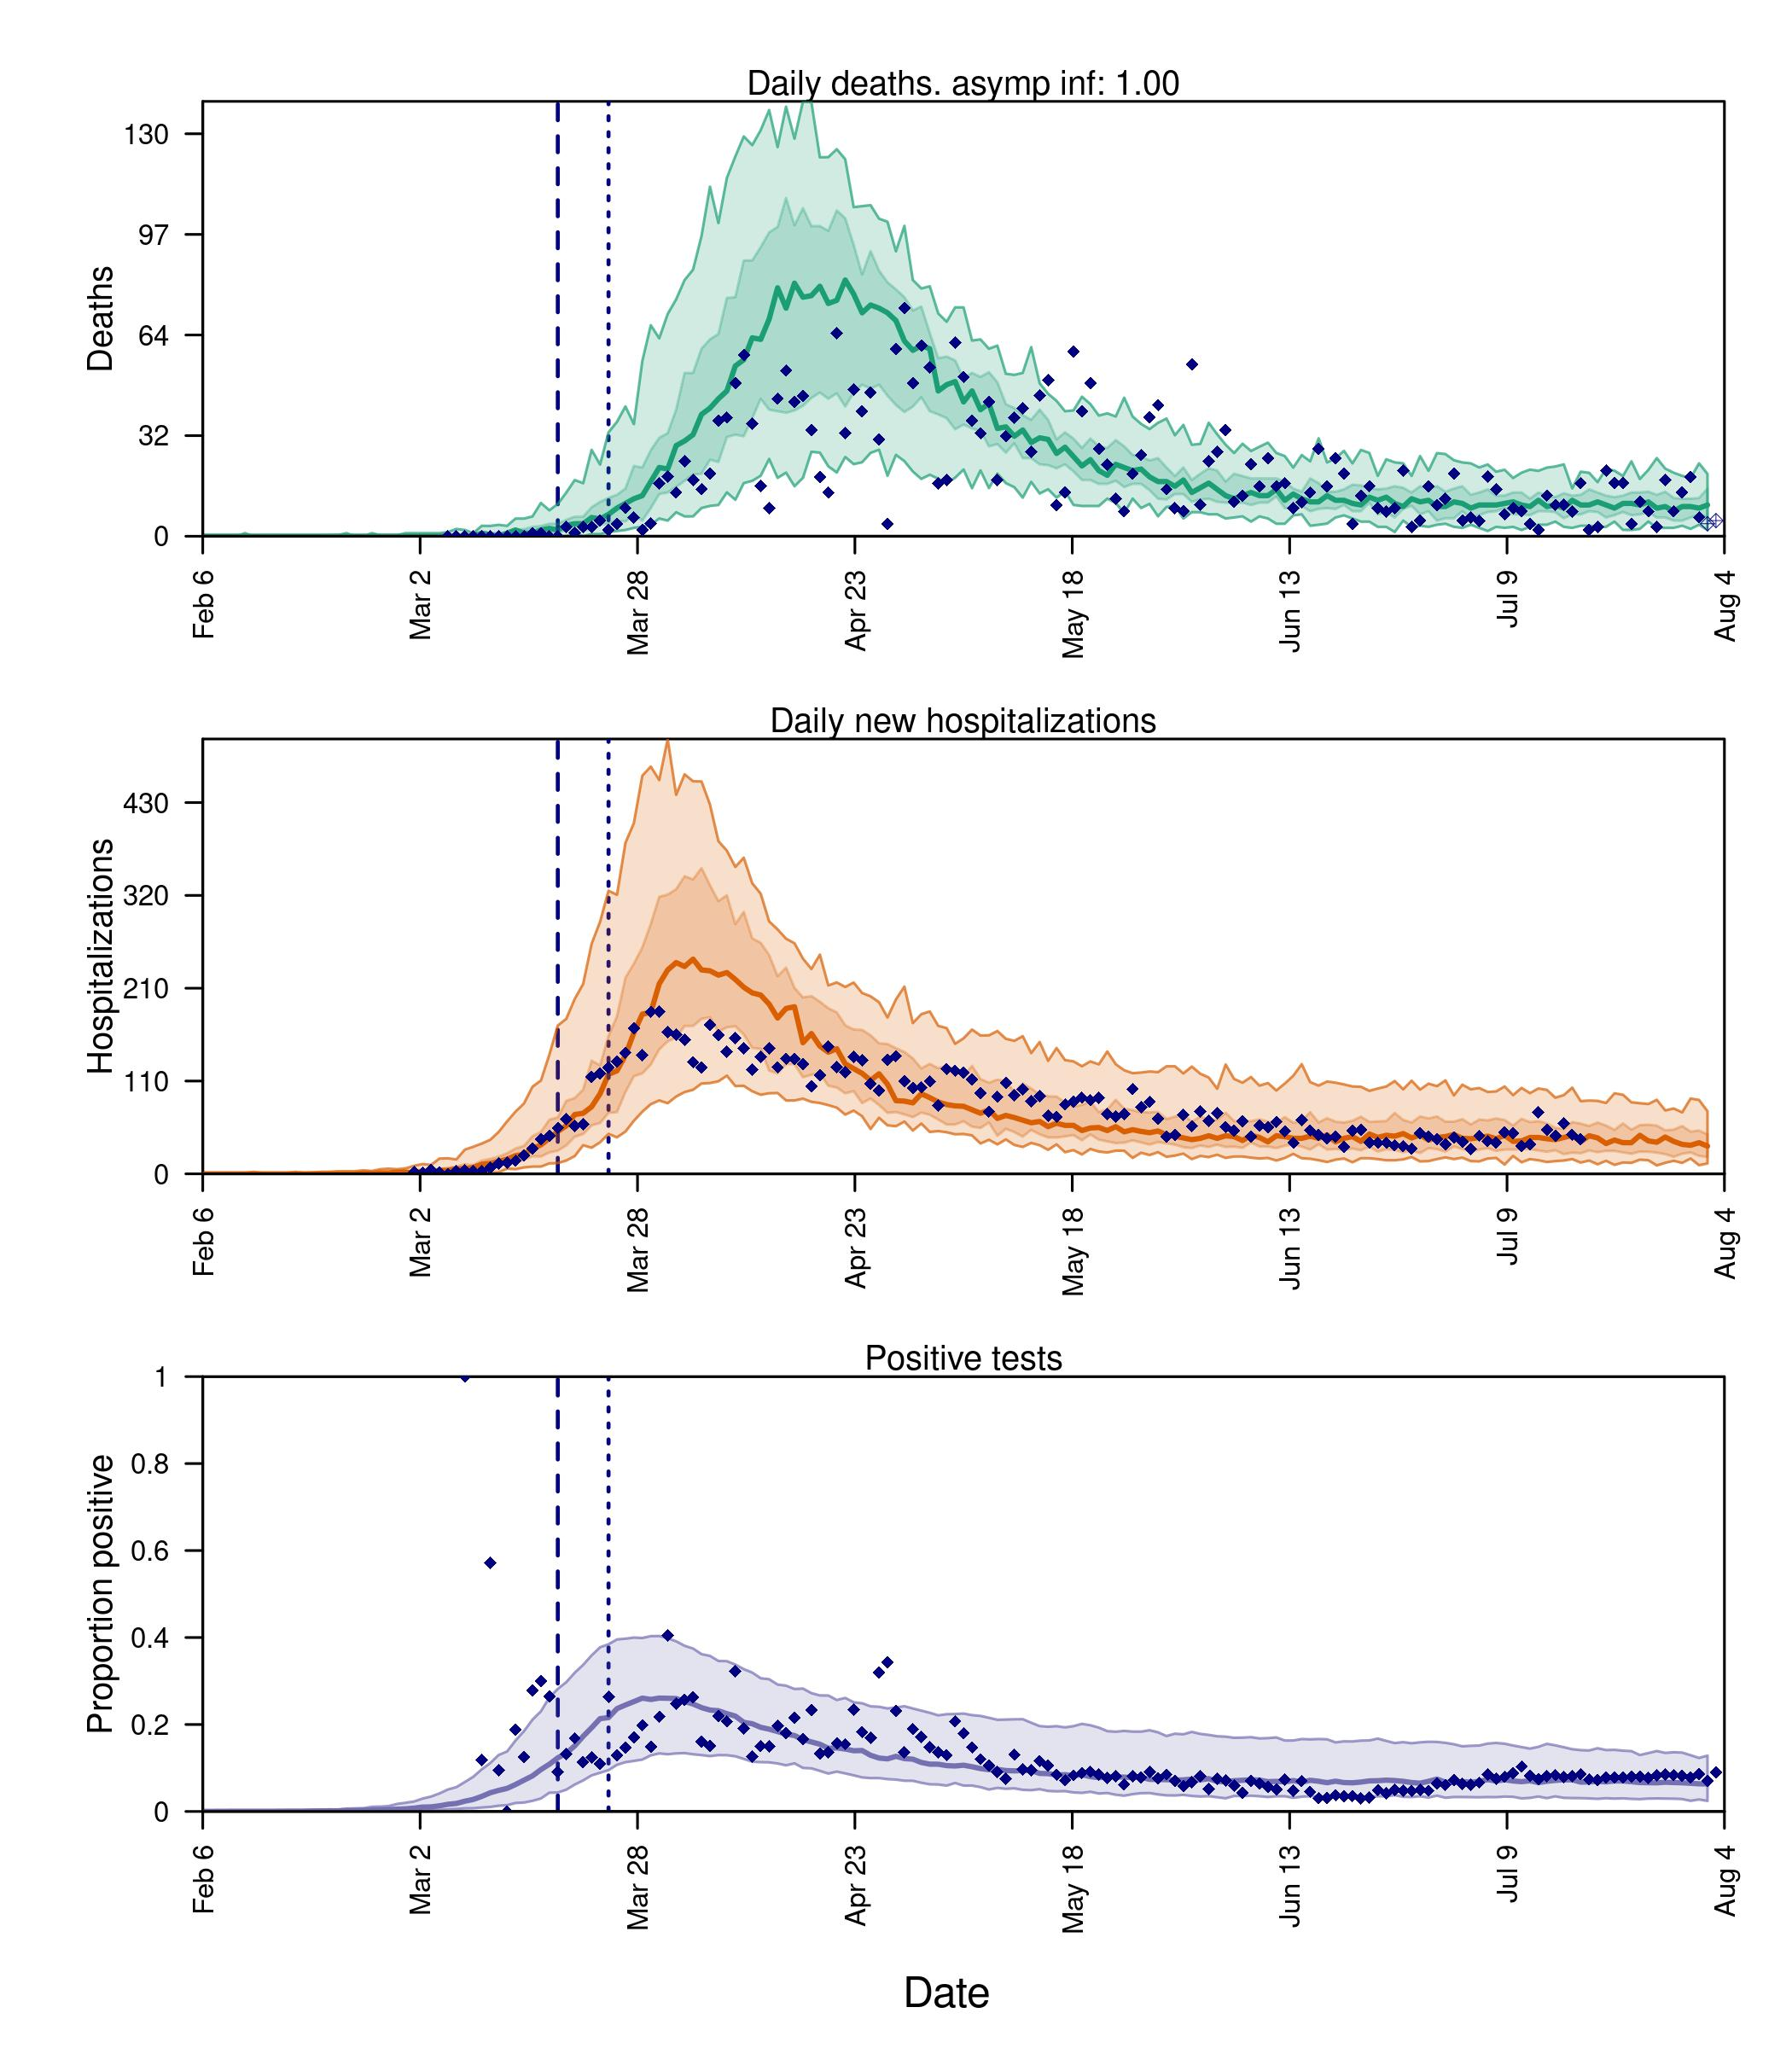
\includegraphics[height=0.8\textheight]{./figures/manuscript_figure_deaths_fit.jpeg}
  \end{figure}
\end{frame}


% =============================================================================%
\begin{frame}
  \frametitle{Future work}
  \begin{itemize}
  \item Adding face-masks to improve fit.
  \item We are using this model to assess school reopening scenarios in Indiana.
  \end{itemize}    
\end{frame}

% =============================================================================%
\begin{frame}
  \frametitle{Funding statement}
  This research is being funded by an NSF RAPID grant: Real-time updating of an agent-based model to inform COVID-19 mitigation strategies. Award number: 2027718.
\end{frame}

% =============================================================================%
\begin{frame}[t,allowframebreaks]
  \frametitle{References}
  \printbibliography
  %\bibliography{Guido_Postdoc_Literature}
\end{frame}
% \bibliographystyle{apalike}

\end{document}


%%% Local Variables:
%%% mode: latex
%%% TeX-master: t
%%% End:
